% Created by tikzDevice version 0.7.0 on 2014-06-29 19:47:43
% !TEX encoding = UTF-8 Unicode
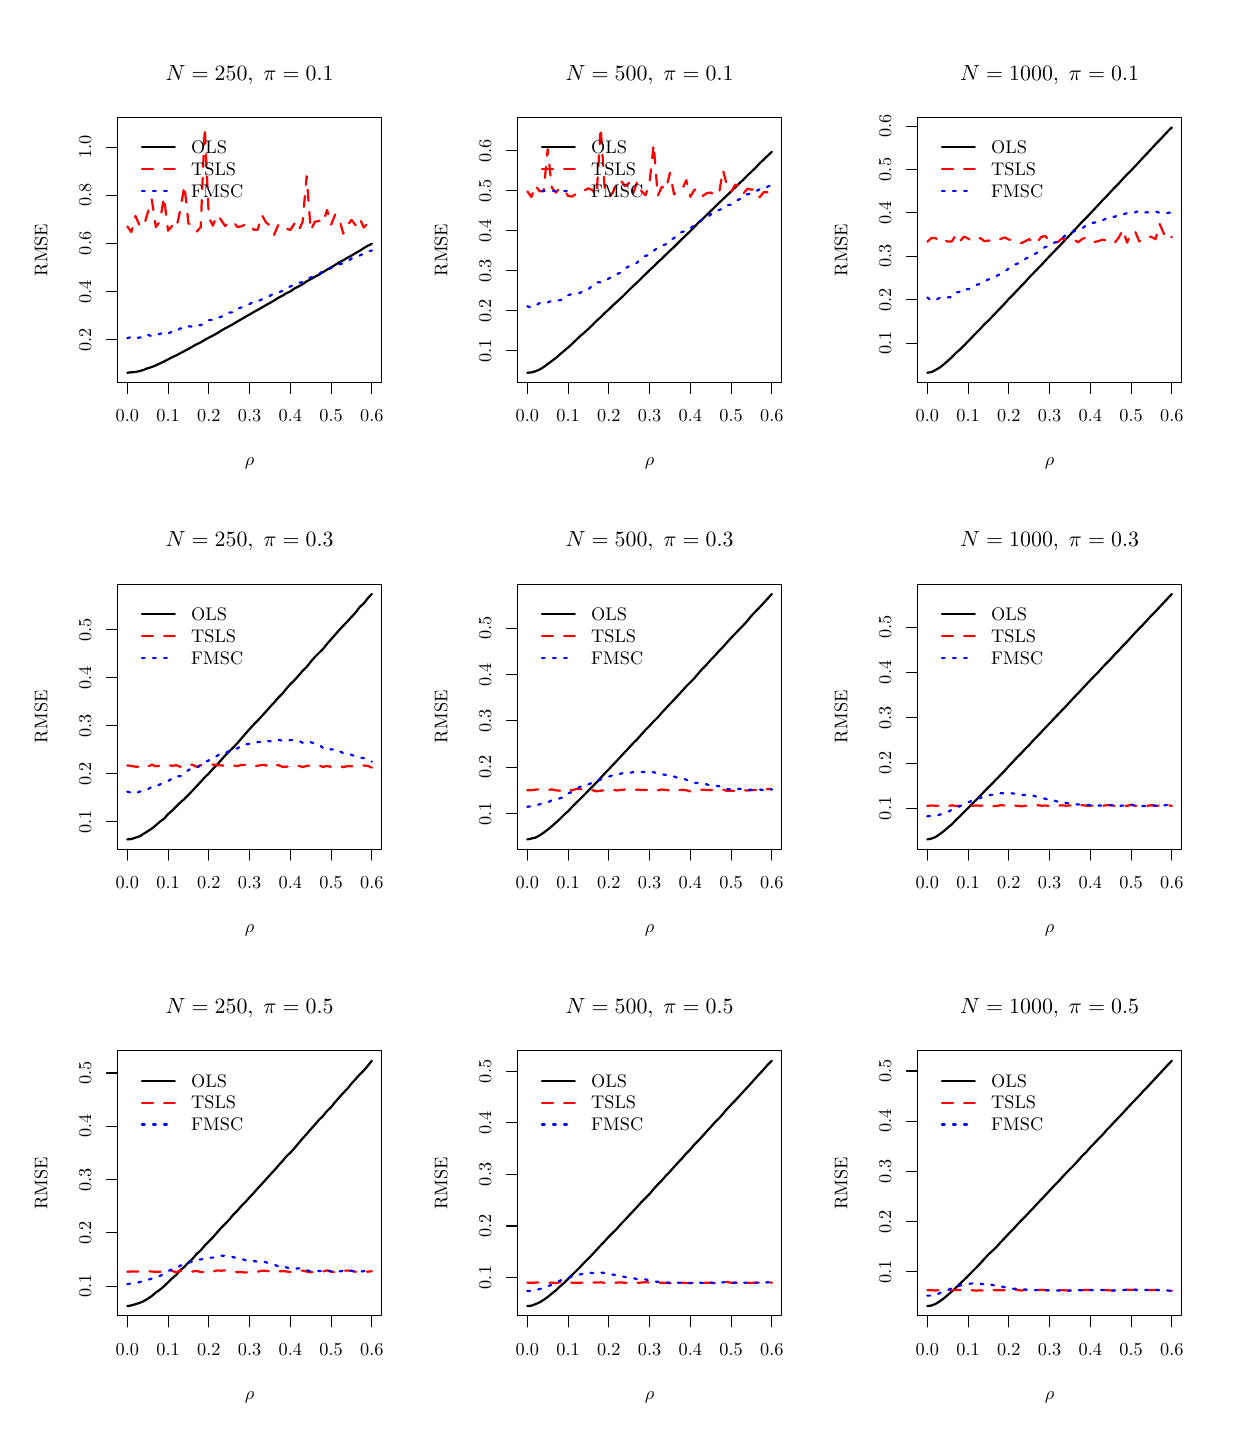
\begin{tikzpicture}[x=1pt,y=1pt]
\definecolor[named]{fillColor}{rgb}{1.00,1.00,1.00}
\path[use as bounding box,fill=fillColor,fill opacity=0.00] (0,0) rectangle (433.62,505.89);
\begin{scope}
\path[clip] ( 32.47,377.65) rectangle (127.91,473.42);
\definecolor[named]{drawColor}{rgb}{0.00,0.00,0.00}

\path[draw=drawColor,line width= 0.8pt,line join=round,line cap=round] ( 36.01,381.20) --
	( 37.48,381.35) --
	( 38.95,381.47) --
	( 40.42,381.79) --
	( 41.90,382.22) --
	( 43.37,382.82) --
	( 44.84,383.26) --
	( 46.32,383.86) --
	( 47.79,384.56) --
	( 49.26,385.24) --
	( 50.73,386.01) --
	( 52.21,386.80) --
	( 53.68,387.44) --
	( 55.15,388.26) --
	( 56.63,389.02) --
	( 58.10,389.82) --
	( 59.57,390.64) --
	( 61.04,391.49) --
	( 62.52,392.14) --
	( 63.99,393.10) --
	( 65.46,393.86) --
	( 66.93,394.61) --
	( 68.41,395.43) --
	( 69.88,396.38) --
	( 71.35,397.22) --
	( 72.83,398.01) --
	( 74.30,398.81) --
	( 75.77,399.71) --
	( 77.24,400.55) --
	( 78.72,401.42) --
	( 80.19,402.24) --
	( 81.66,403.10) --
	( 83.14,403.93) --
	( 84.61,404.75) --
	( 86.08,405.60) --
	( 87.55,406.42) --
	( 89.03,407.28) --
	( 90.50,408.25) --
	( 91.97,408.98) --
	( 93.44,409.91) --
	( 94.92,410.58) --
	( 96.39,411.63) --
	( 97.86,412.36) --
	( 99.34,413.17) --
	(100.81,414.21) --
	(102.28,414.99) --
	(103.75,415.84) --
	(105.23,416.61) --
	(106.70,417.54) --
	(108.17,418.46) --
	(109.65,419.27) --
	(111.12,420.15) --
	(112.59,421.11) --
	(114.06,421.82) --
	(115.54,422.75) --
	(117.01,423.53) --
	(118.48,424.43) --
	(119.95,425.24) --
	(121.43,426.21) --
	(122.90,427.09) --
	(124.37,427.80);
\end{scope}
\begin{scope}
\path[clip] (  0.00,  0.00) rectangle (433.62,505.89);
\definecolor[named]{drawColor}{rgb}{0.00,0.00,0.00}

\path[draw=drawColor,line width= 0.4pt,line join=round,line cap=round] ( 36.01,377.65) -- (124.37,377.65);

\path[draw=drawColor,line width= 0.4pt,line join=round,line cap=round] ( 36.01,377.65) -- ( 36.01,373.69);

\path[draw=drawColor,line width= 0.4pt,line join=round,line cap=round] ( 50.73,377.65) -- ( 50.73,373.69);

\path[draw=drawColor,line width= 0.4pt,line join=round,line cap=round] ( 65.46,377.65) -- ( 65.46,373.69);

\path[draw=drawColor,line width= 0.4pt,line join=round,line cap=round] ( 80.19,377.65) -- ( 80.19,373.69);

\path[draw=drawColor,line width= 0.4pt,line join=round,line cap=round] ( 94.92,377.65) -- ( 94.92,373.69);

\path[draw=drawColor,line width= 0.4pt,line join=round,line cap=round] (109.65,377.65) -- (109.65,373.69);

\path[draw=drawColor,line width= 0.4pt,line join=round,line cap=round] (124.37,377.65) -- (124.37,373.69);

\node[text=drawColor,anchor=base,inner sep=0pt, outer sep=0pt, scale=  0.66] at ( 36.01,363.40) {0.0};

\node[text=drawColor,anchor=base,inner sep=0pt, outer sep=0pt, scale=  0.66] at ( 50.73,363.40) {0.1};

\node[text=drawColor,anchor=base,inner sep=0pt, outer sep=0pt, scale=  0.66] at ( 65.46,363.40) {0.2};

\node[text=drawColor,anchor=base,inner sep=0pt, outer sep=0pt, scale=  0.66] at ( 80.19,363.40) {0.3};

\node[text=drawColor,anchor=base,inner sep=0pt, outer sep=0pt, scale=  0.66] at ( 94.92,363.40) {0.4};

\node[text=drawColor,anchor=base,inner sep=0pt, outer sep=0pt, scale=  0.66] at (109.65,363.40) {0.5};

\node[text=drawColor,anchor=base,inner sep=0pt, outer sep=0pt, scale=  0.66] at (124.37,363.40) {0.6};

\path[draw=drawColor,line width= 0.4pt,line join=round,line cap=round] ( 32.47,393.12) -- ( 32.47,462.73);

\path[draw=drawColor,line width= 0.4pt,line join=round,line cap=round] ( 32.47,393.12) -- ( 28.51,393.12);

\path[draw=drawColor,line width= 0.4pt,line join=round,line cap=round] ( 32.47,410.52) -- ( 28.51,410.52);

\path[draw=drawColor,line width= 0.4pt,line join=round,line cap=round] ( 32.47,427.92) -- ( 28.51,427.92);

\path[draw=drawColor,line width= 0.4pt,line join=round,line cap=round] ( 32.47,445.33) -- ( 28.51,445.33);

\path[draw=drawColor,line width= 0.4pt,line join=round,line cap=round] ( 32.47,462.73) -- ( 28.51,462.73);

\node[text=drawColor,rotate= 90.00,anchor=base,inner sep=0pt, outer sep=0pt, scale=  0.66] at ( 22.97,393.12) {0.2};

\node[text=drawColor,rotate= 90.00,anchor=base,inner sep=0pt, outer sep=0pt, scale=  0.66] at ( 22.97,410.52) {0.4};

\node[text=drawColor,rotate= 90.00,anchor=base,inner sep=0pt, outer sep=0pt, scale=  0.66] at ( 22.97,427.92) {0.6};

\node[text=drawColor,rotate= 90.00,anchor=base,inner sep=0pt, outer sep=0pt, scale=  0.66] at ( 22.97,445.33) {0.8};

\node[text=drawColor,rotate= 90.00,anchor=base,inner sep=0pt, outer sep=0pt, scale=  0.66] at ( 22.97,462.73) {1.0};

\path[draw=drawColor,line width= 0.4pt,line join=round,line cap=round] ( 32.47,377.65) --
	(127.91,377.65) --
	(127.91,473.42) --
	( 32.47,473.42) --
	( 32.47,377.65);
\end{scope}
\begin{scope}
\path[clip] (  0.00,337.26) rectangle (144.54,505.89);
\definecolor[named]{drawColor}{rgb}{0.00,0.00,0.00}

\node[text=drawColor,anchor=base,inner sep=0pt, outer sep=0pt, scale=  0.79] at ( 80.19,486.92) {\bfseries $N=250, \;\pi=0.1$};

\node[text=drawColor,anchor=base,inner sep=0pt, outer sep=0pt, scale=  0.66] at ( 80.19,347.56) {$\rho$};

\node[text=drawColor,rotate= 90.00,anchor=base,inner sep=0pt, outer sep=0pt, scale=  0.66] at (  7.13,425.53) {RMSE};
\end{scope}
\begin{scope}
\path[clip] ( 32.47,377.65) rectangle (127.91,473.42);
\definecolor[named]{drawColor}{rgb}{1.00,0.00,0.00}

\path[draw=drawColor,line width= 0.8pt,dash pattern=on 4pt off 4pt ,line join=round,line cap=round] ( 36.01,434.07) --
	( 37.48,432.02) --
	( 38.95,437.88) --
	( 40.42,434.44) --
	( 41.90,433.98) --
	( 43.37,438.95) --
	( 44.84,443.84) --
	( 46.32,433.86) --
	( 47.79,435.87) --
	( 49.26,444.60) --
	( 50.73,432.52) --
	( 52.21,434.26) --
	( 53.68,433.26) --
	( 55.15,439.98) --
	( 56.63,448.90) --
	( 58.10,435.16) --
	( 59.57,434.51) --
	( 61.04,432.14) --
	( 62.52,433.74) --
	( 63.99,469.87) --
	( 65.46,437.24) --
	( 66.93,434.33) --
	( 68.41,438.23) --
	( 69.88,436.44) --
	( 71.35,434.23) --
	( 72.83,435.42) --
	( 74.30,435.89) --
	( 75.77,433.86) --
	( 77.24,434.11) --
	( 78.72,434.78) --
	( 80.19,435.06) --
	( 81.66,432.84) --
	( 83.14,432.89) --
	( 84.61,438.20) --
	( 86.08,435.59) --
	( 87.55,434.30) --
	( 89.03,431.04) --
	( 90.50,434.50) --
	( 91.97,432.79) --
	( 93.44,433.24) --
	( 94.92,432.78) --
	( 96.39,435.06) --
	( 97.86,432.41) --
	( 99.34,435.71) --
	(100.81,452.19) --
	(102.28,432.61) --
	(103.75,435.73) --
	(105.23,436.06) --
	(106.70,435.26) --
	(108.17,440.04) --
	(109.65,434.64) --
	(111.12,438.41) --
	(112.59,436.68) --
	(114.06,431.46) --
	(115.54,434.41) --
	(117.01,436.42) --
	(118.48,434.53) --
	(119.95,437.08) --
	(121.43,433.66) --
	(122.90,435.23) --
	(124.37,434.04);
\definecolor[named]{drawColor}{rgb}{0.00,0.00,1.00}

\path[draw=drawColor,line width= 0.8pt,dash pattern=on 1pt off 3pt ,line join=round,line cap=round] ( 36.01,393.67) --
	( 37.48,394.15) --
	( 38.95,393.60) --
	( 40.42,393.94) --
	( 41.90,394.08) --
	( 43.37,394.96) --
	( 44.84,394.39) --
	( 46.32,394.94) --
	( 47.79,395.21) --
	( 49.26,395.97) --
	( 50.73,395.44) --
	( 52.21,396.01) --
	( 53.68,396.00) --
	( 55.15,397.24) --
	( 56.63,397.02) --
	( 58.10,397.99) --
	( 59.57,397.85) --
	( 61.04,398.48) --
	( 62.52,398.37) --
	( 63.99,399.33) --
	( 65.46,400.22) --
	( 66.93,400.24) --
	( 68.41,400.99) --
	( 69.88,401.42) --
	( 71.35,402.15) --
	( 72.83,402.97) --
	( 74.30,403.02) --
	( 75.77,404.28) --
	( 77.24,404.81) --
	( 78.72,405.44) --
	( 80.19,406.03) --
	( 81.66,406.92) --
	( 83.14,406.99) --
	( 84.61,407.71) --
	( 86.08,408.58) --
	( 87.55,409.00) --
	( 89.03,409.85) --
	( 90.50,410.18) --
	( 91.97,410.72) --
	( 93.44,411.76) --
	( 94.92,412.40) --
	( 96.39,412.89) --
	( 97.86,413.65) --
	( 99.34,413.92) --
	(100.81,415.08) --
	(102.28,415.60) --
	(103.75,416.42) --
	(105.23,416.86) --
	(106.70,417.88) --
	(108.17,418.29) --
	(109.65,419.03) --
	(111.12,419.72) --
	(112.59,420.39) --
	(114.06,420.72) --
	(115.54,421.51) --
	(117.01,422.45) --
	(118.48,422.94) --
	(119.95,423.54) --
	(121.43,424.26) --
	(122.90,425.01) --
	(124.37,425.36);
\definecolor[named]{drawColor}{rgb}{0.00,0.00,0.00}

\path[draw=drawColor,line width= 0.8pt,line join=round,line cap=round] ( 41.28,462.63) -- ( 53.16,462.63);
\definecolor[named]{drawColor}{rgb}{1.00,0.00,0.00}

\path[draw=drawColor,line width= 0.8pt,dash pattern=on 4pt off 4pt ,line join=round,line cap=round] ( 41.28,454.71) -- ( 53.16,454.71);
\definecolor[named]{drawColor}{rgb}{0.00,0.00,1.00}

\path[draw=drawColor,line width= 0.8pt,dash pattern=on 1pt off 3pt ,line join=round,line cap=round] ( 41.28,446.79) -- ( 53.16,446.79);
\definecolor[named]{drawColor}{rgb}{0.00,0.00,0.00}

\node[text=drawColor,anchor=base west,inner sep=0pt, outer sep=0pt, scale=  0.66] at ( 59.10,460.35) {OLS};

\node[text=drawColor,anchor=base west,inner sep=0pt, outer sep=0pt, scale=  0.66] at ( 59.10,452.43) {TSLS};

\node[text=drawColor,anchor=base west,inner sep=0pt, outer sep=0pt, scale=  0.66] at ( 59.10,444.51) {FMSC};
\end{scope}
\begin{scope}
\path[clip] (177.01,377.65) rectangle (272.45,473.42);
\definecolor[named]{drawColor}{rgb}{0.00,0.00,0.00}

\path[draw=drawColor,line width= 0.8pt,line join=round,line cap=round] (180.55,381.20) --
	(182.02,381.31) --
	(183.49,381.73) --
	(184.96,382.35) --
	(186.44,383.24) --
	(187.91,384.35) --
	(189.38,385.42) --
	(190.86,386.52) --
	(192.33,387.84) --
	(193.80,389.07) --
	(195.27,390.31) --
	(196.75,391.64) --
	(198.22,393.08) --
	(199.69,394.47) --
	(201.17,395.72) --
	(202.64,397.07) --
	(204.11,398.47) --
	(205.58,399.99) --
	(207.06,401.27) --
	(208.53,402.79) --
	(210.00,404.09) --
	(211.47,405.56) --
	(212.95,406.85) --
	(214.42,408.21) --
	(215.89,409.64) --
	(217.37,411.15) --
	(218.84,412.56) --
	(220.31,413.91) --
	(221.78,415.37) --
	(223.26,416.81) --
	(224.73,418.29) --
	(226.20,419.58) --
	(227.68,421.12) --
	(229.15,422.42) --
	(230.62,423.86) --
	(232.09,425.31) --
	(233.57,426.65) --
	(235.04,428.14) --
	(236.51,429.59) --
	(237.98,430.99) --
	(239.46,432.39) --
	(240.93,433.89) --
	(242.40,435.47) --
	(243.88,436.73) --
	(245.35,438.20) --
	(246.82,439.63) --
	(248.29,441.04) --
	(249.77,442.53) --
	(251.24,443.90) --
	(252.71,445.30) --
	(254.19,446.71) --
	(255.66,448.13) --
	(257.13,449.62) --
	(258.60,450.93) --
	(260.08,452.49) --
	(261.55,453.87) --
	(263.02,455.25) --
	(264.50,456.86) --
	(265.97,458.24) --
	(267.44,459.68) --
	(268.91,461.04);
\end{scope}
\begin{scope}
\path[clip] (  0.00,  0.00) rectangle (433.62,505.89);
\definecolor[named]{drawColor}{rgb}{0.00,0.00,0.00}

\path[draw=drawColor,line width= 0.4pt,line join=round,line cap=round] (180.55,377.65) -- (268.91,377.65);

\path[draw=drawColor,line width= 0.4pt,line join=round,line cap=round] (180.55,377.65) -- (180.55,373.69);

\path[draw=drawColor,line width= 0.4pt,line join=round,line cap=round] (195.27,377.65) -- (195.27,373.69);

\path[draw=drawColor,line width= 0.4pt,line join=round,line cap=round] (210.00,377.65) -- (210.00,373.69);

\path[draw=drawColor,line width= 0.4pt,line join=round,line cap=round] (224.73,377.65) -- (224.73,373.69);

\path[draw=drawColor,line width= 0.4pt,line join=round,line cap=round] (239.46,377.65) -- (239.46,373.69);

\path[draw=drawColor,line width= 0.4pt,line join=round,line cap=round] (254.19,377.65) -- (254.19,373.69);

\path[draw=drawColor,line width= 0.4pt,line join=round,line cap=round] (268.91,377.65) -- (268.91,373.69);

\node[text=drawColor,anchor=base,inner sep=0pt, outer sep=0pt, scale=  0.66] at (180.55,363.40) {0.0};

\node[text=drawColor,anchor=base,inner sep=0pt, outer sep=0pt, scale=  0.66] at (195.27,363.40) {0.1};

\node[text=drawColor,anchor=base,inner sep=0pt, outer sep=0pt, scale=  0.66] at (210.00,363.40) {0.2};

\node[text=drawColor,anchor=base,inner sep=0pt, outer sep=0pt, scale=  0.66] at (224.73,363.40) {0.3};

\node[text=drawColor,anchor=base,inner sep=0pt, outer sep=0pt, scale=  0.66] at (239.46,363.40) {0.4};

\node[text=drawColor,anchor=base,inner sep=0pt, outer sep=0pt, scale=  0.66] at (254.19,363.40) {0.5};

\node[text=drawColor,anchor=base,inner sep=0pt, outer sep=0pt, scale=  0.66] at (268.91,363.40) {0.6};

\path[draw=drawColor,line width= 0.4pt,line join=round,line cap=round] (177.01,389.08) -- (177.01,461.34);

\path[draw=drawColor,line width= 0.4pt,line join=round,line cap=round] (177.01,389.08) -- (173.05,389.08);

\path[draw=drawColor,line width= 0.4pt,line join=round,line cap=round] (177.01,403.53) -- (173.05,403.53);

\path[draw=drawColor,line width= 0.4pt,line join=round,line cap=round] (177.01,417.98) -- (173.05,417.98);

\path[draw=drawColor,line width= 0.4pt,line join=round,line cap=round] (177.01,432.44) -- (173.05,432.44);

\path[draw=drawColor,line width= 0.4pt,line join=round,line cap=round] (177.01,446.89) -- (173.05,446.89);

\path[draw=drawColor,line width= 0.4pt,line join=round,line cap=round] (177.01,461.34) -- (173.05,461.34);

\node[text=drawColor,rotate= 90.00,anchor=base,inner sep=0pt, outer sep=0pt, scale=  0.66] at (167.51,389.08) {0.1};

\node[text=drawColor,rotate= 90.00,anchor=base,inner sep=0pt, outer sep=0pt, scale=  0.66] at (167.51,403.53) {0.2};

\node[text=drawColor,rotate= 90.00,anchor=base,inner sep=0pt, outer sep=0pt, scale=  0.66] at (167.51,417.98) {0.3};

\node[text=drawColor,rotate= 90.00,anchor=base,inner sep=0pt, outer sep=0pt, scale=  0.66] at (167.51,432.44) {0.4};

\node[text=drawColor,rotate= 90.00,anchor=base,inner sep=0pt, outer sep=0pt, scale=  0.66] at (167.51,446.89) {0.5};

\node[text=drawColor,rotate= 90.00,anchor=base,inner sep=0pt, outer sep=0pt, scale=  0.66] at (167.51,461.34) {0.6};

\path[draw=drawColor,line width= 0.4pt,line join=round,line cap=round] (177.01,377.65) --
	(272.45,377.65) --
	(272.45,473.42) --
	(177.01,473.42) --
	(177.01,377.65);
\end{scope}
\begin{scope}
\path[clip] (144.54,337.26) rectangle (289.08,505.89);
\definecolor[named]{drawColor}{rgb}{0.00,0.00,0.00}

\node[text=drawColor,anchor=base,inner sep=0pt, outer sep=0pt, scale=  0.79] at (224.73,486.92) {\bfseries $N=500, \;\pi=0.1$};

\node[text=drawColor,anchor=base,inner sep=0pt, outer sep=0pt, scale=  0.66] at (224.73,347.56) {$\rho$};

\node[text=drawColor,rotate= 90.00,anchor=base,inner sep=0pt, outer sep=0pt, scale=  0.66] at (151.67,425.53) {RMSE};
\end{scope}
\begin{scope}
\path[clip] (177.01,377.65) rectangle (272.45,473.42);
\definecolor[named]{drawColor}{rgb}{1.00,0.00,0.00}

\path[draw=drawColor,line width= 0.8pt,dash pattern=on 4pt off 4pt ,line join=round,line cap=round] (180.55,446.73) --
	(182.02,444.70) --
	(183.49,448.95) --
	(184.96,446.76) --
	(186.44,446.76) --
	(187.91,461.99) --
	(189.38,448.16) --
	(190.86,446.30) --
	(192.33,447.86) --
	(193.80,447.41) --
	(195.27,445.06) --
	(196.75,444.86) --
	(198.22,445.85) --
	(199.69,445.86) --
	(201.17,447.10) --
	(202.64,447.85) --
	(204.11,447.14) --
	(205.58,445.29) --
	(207.06,469.87) --
	(208.53,447.40) --
	(210.00,444.73) --
	(211.47,446.28) --
	(212.95,450.54) --
	(214.42,450.50) --
	(215.89,448.63) --
	(217.37,449.81) --
	(218.84,446.13) --
	(220.31,450.33) --
	(221.78,446.83) --
	(223.26,445.33) --
	(224.73,450.08) --
	(226.20,463.70) --
	(227.68,445.05) --
	(229.15,448.44) --
	(230.62,447.31) --
	(232.09,453.44) --
	(233.57,445.67) --
	(235.04,446.87) --
	(236.51,447.46) --
	(237.98,450.76) --
	(239.46,444.80) --
	(240.93,447.32) --
	(242.40,447.57) --
	(243.88,445.06) --
	(245.35,446.06) --
	(246.82,446.31) --
	(248.29,445.39) --
	(249.77,445.65) --
	(251.24,454.42) --
	(252.71,448.74) --
	(254.19,446.56) --
	(255.66,449.14) --
	(257.13,448.77) --
	(258.60,445.89) --
	(260.08,447.72) --
	(261.55,447.35) --
	(263.02,447.49) --
	(264.50,444.59) --
	(265.97,446.43) --
	(267.44,446.38) --
	(268.91,445.57);
\definecolor[named]{drawColor}{rgb}{0.00,0.00,1.00}

\path[draw=drawColor,line width= 0.8pt,dash pattern=on 1pt off 3pt ,line join=round,line cap=round] (180.55,405.22) --
	(182.02,404.72) --
	(183.49,405.42) --
	(184.96,406.35) --
	(186.44,406.26) --
	(187.91,406.62) --
	(189.38,407.20) --
	(190.86,407.25) --
	(192.33,407.40) --
	(193.80,408.03) --
	(195.27,409.20) --
	(196.75,409.68) --
	(198.22,409.88) --
	(199.69,410.07) --
	(201.17,411.19) --
	(202.64,411.36) --
	(204.11,412.73) --
	(205.58,413.86) --
	(207.06,413.87) --
	(208.53,414.18) --
	(210.00,415.26) --
	(211.47,416.00) --
	(212.95,416.90) --
	(214.42,417.35) --
	(215.89,418.91) --
	(217.37,419.72) --
	(218.84,420.19) --
	(220.31,421.07) --
	(221.78,422.55) --
	(223.26,423.44) --
	(224.73,423.82) --
	(226.20,425.24) --
	(227.68,426.36) --
	(229.15,427.13) --
	(230.62,427.63) --
	(232.09,429.15) --
	(233.57,429.84) --
	(235.04,431.35) --
	(236.51,432.10) --
	(237.98,432.34) --
	(239.46,433.40) --
	(240.93,434.49) --
	(242.40,435.38) --
	(243.88,436.62) --
	(245.35,437.01) --
	(246.82,438.44) --
	(248.29,438.78) --
	(249.77,439.98) --
	(251.24,440.51) --
	(252.71,441.73) --
	(254.19,441.92) --
	(255.66,443.02) --
	(257.13,443.88) --
	(258.60,444.39) --
	(260.08,445.75) --
	(261.55,445.89) --
	(263.02,446.64) --
	(264.50,447.54) --
	(265.97,447.56) --
	(267.44,448.46) --
	(268.91,449.10);
\definecolor[named]{drawColor}{rgb}{0.00,0.00,0.00}

\path[draw=drawColor,line width= 0.8pt,line join=round,line cap=round] (185.82,462.63) -- (197.70,462.63);
\definecolor[named]{drawColor}{rgb}{1.00,0.00,0.00}

\path[draw=drawColor,line width= 0.8pt,dash pattern=on 4pt off 4pt ,line join=round,line cap=round] (185.82,454.71) -- (197.70,454.71);
\definecolor[named]{drawColor}{rgb}{0.00,0.00,1.00}

\path[draw=drawColor,line width= 0.8pt,dash pattern=on 1pt off 3pt ,line join=round,line cap=round] (185.82,446.79) -- (197.70,446.79);
\definecolor[named]{drawColor}{rgb}{0.00,0.00,0.00}

\node[text=drawColor,anchor=base west,inner sep=0pt, outer sep=0pt, scale=  0.66] at (203.64,460.35) {OLS};

\node[text=drawColor,anchor=base west,inner sep=0pt, outer sep=0pt, scale=  0.66] at (203.64,452.43) {TSLS};

\node[text=drawColor,anchor=base west,inner sep=0pt, outer sep=0pt, scale=  0.66] at (203.64,444.51) {FMSC};
\end{scope}
\begin{scope}
\path[clip] (321.55,377.65) rectangle (416.99,473.42);
\definecolor[named]{drawColor}{rgb}{0.00,0.00,0.00}

\path[draw=drawColor,line width= 0.8pt,line join=round,line cap=round] (325.09,381.20) --
	(326.56,381.44) --
	(328.03,382.17) --
	(329.50,383.02) --
	(330.98,384.18) --
	(332.45,385.45) --
	(333.92,386.78) --
	(335.40,388.34) --
	(336.87,389.58) --
	(338.34,391.06) --
	(339.81,392.54) --
	(341.29,394.09) --
	(342.76,395.62) --
	(344.23,397.08) --
	(345.71,398.71) --
	(347.18,400.04) --
	(348.65,401.61) --
	(350.12,403.14) --
	(351.60,404.69) --
	(353.07,406.21) --
	(354.54,407.91) --
	(356.01,409.33) --
	(357.49,410.91) --
	(358.96,412.49) --
	(360.43,413.95) --
	(361.91,415.65) --
	(363.38,417.13) --
	(364.85,418.65) --
	(366.32,420.17) --
	(367.80,421.77) --
	(369.27,423.33) --
	(370.74,424.85) --
	(372.22,426.36) --
	(373.69,427.88) --
	(375.16,429.47) --
	(376.63,431.00) --
	(378.11,432.62) --
	(379.58,434.16) --
	(381.05,435.78) --
	(382.52,437.19) --
	(384.00,438.77) --
	(385.47,440.35) --
	(386.94,441.92) --
	(388.42,443.52) --
	(389.89,444.99) --
	(391.36,446.62) --
	(392.83,448.16) --
	(394.31,449.65) --
	(395.78,451.29) --
	(397.25,452.86) --
	(398.73,454.27) --
	(400.20,455.88) --
	(401.67,457.44) --
	(403.14,459.03) --
	(404.62,460.58) --
	(406.09,462.17) --
	(407.56,463.77) --
	(409.04,465.25) --
	(410.51,466.85) --
	(411.98,468.42) --
	(413.45,469.87);
\end{scope}
\begin{scope}
\path[clip] (  0.00,  0.00) rectangle (433.62,505.89);
\definecolor[named]{drawColor}{rgb}{0.00,0.00,0.00}

\path[draw=drawColor,line width= 0.4pt,line join=round,line cap=round] (325.09,377.65) -- (413.45,377.65);

\path[draw=drawColor,line width= 0.4pt,line join=round,line cap=round] (325.09,377.65) -- (325.09,373.69);

\path[draw=drawColor,line width= 0.4pt,line join=round,line cap=round] (339.81,377.65) -- (339.81,373.69);

\path[draw=drawColor,line width= 0.4pt,line join=round,line cap=round] (354.54,377.65) -- (354.54,373.69);

\path[draw=drawColor,line width= 0.4pt,line join=round,line cap=round] (369.27,377.65) -- (369.27,373.69);

\path[draw=drawColor,line width= 0.4pt,line join=round,line cap=round] (384.00,377.65) -- (384.00,373.69);

\path[draw=drawColor,line width= 0.4pt,line join=round,line cap=round] (398.73,377.65) -- (398.73,373.69);

\path[draw=drawColor,line width= 0.4pt,line join=round,line cap=round] (413.45,377.65) -- (413.45,373.69);

\node[text=drawColor,anchor=base,inner sep=0pt, outer sep=0pt, scale=  0.66] at (325.09,363.40) {0.0};

\node[text=drawColor,anchor=base,inner sep=0pt, outer sep=0pt, scale=  0.66] at (339.81,363.40) {0.1};

\node[text=drawColor,anchor=base,inner sep=0pt, outer sep=0pt, scale=  0.66] at (354.54,363.40) {0.2};

\node[text=drawColor,anchor=base,inner sep=0pt, outer sep=0pt, scale=  0.66] at (369.27,363.40) {0.3};

\node[text=drawColor,anchor=base,inner sep=0pt, outer sep=0pt, scale=  0.66] at (384.00,363.40) {0.4};

\node[text=drawColor,anchor=base,inner sep=0pt, outer sep=0pt, scale=  0.66] at (398.73,363.40) {0.5};

\node[text=drawColor,anchor=base,inner sep=0pt, outer sep=0pt, scale=  0.66] at (413.45,363.40) {0.6};

\path[draw=drawColor,line width= 0.4pt,line join=round,line cap=round] (321.55,391.91) -- (321.55,470.33);

\path[draw=drawColor,line width= 0.4pt,line join=round,line cap=round] (321.55,391.91) -- (317.59,391.91);

\path[draw=drawColor,line width= 0.4pt,line join=round,line cap=round] (321.55,407.59) -- (317.59,407.59);

\path[draw=drawColor,line width= 0.4pt,line join=round,line cap=round] (321.55,423.28) -- (317.59,423.28);

\path[draw=drawColor,line width= 0.4pt,line join=round,line cap=round] (321.55,438.96) -- (317.59,438.96);

\path[draw=drawColor,line width= 0.4pt,line join=round,line cap=round] (321.55,454.65) -- (317.59,454.65);

\path[draw=drawColor,line width= 0.4pt,line join=round,line cap=round] (321.55,470.33) -- (317.59,470.33);

\node[text=drawColor,rotate= 90.00,anchor=base,inner sep=0pt, outer sep=0pt, scale=  0.66] at (312.05,391.91) {0.1};

\node[text=drawColor,rotate= 90.00,anchor=base,inner sep=0pt, outer sep=0pt, scale=  0.66] at (312.05,407.59) {0.2};

\node[text=drawColor,rotate= 90.00,anchor=base,inner sep=0pt, outer sep=0pt, scale=  0.66] at (312.05,423.28) {0.3};

\node[text=drawColor,rotate= 90.00,anchor=base,inner sep=0pt, outer sep=0pt, scale=  0.66] at (312.05,438.96) {0.4};

\node[text=drawColor,rotate= 90.00,anchor=base,inner sep=0pt, outer sep=0pt, scale=  0.66] at (312.05,454.65) {0.5};

\node[text=drawColor,rotate= 90.00,anchor=base,inner sep=0pt, outer sep=0pt, scale=  0.66] at (312.05,470.33) {0.6};

\path[draw=drawColor,line width= 0.4pt,line join=round,line cap=round] (321.55,377.65) --
	(416.99,377.65) --
	(416.99,473.42) --
	(321.55,473.42) --
	(321.55,377.65);
\end{scope}
\begin{scope}
\path[clip] (289.08,337.26) rectangle (433.62,505.89);
\definecolor[named]{drawColor}{rgb}{0.00,0.00,0.00}

\node[text=drawColor,anchor=base,inner sep=0pt, outer sep=0pt, scale=  0.79] at (369.27,486.92) {\bfseries $N=1000, \;\pi=0.1$};

\node[text=drawColor,anchor=base,inner sep=0pt, outer sep=0pt, scale=  0.66] at (369.27,347.56) {$\rho$};

\node[text=drawColor,rotate= 90.00,anchor=base,inner sep=0pt, outer sep=0pt, scale=  0.66] at (296.21,425.53) {RMSE};
\end{scope}
\begin{scope}
\path[clip] (321.55,377.65) rectangle (416.99,473.42);
\definecolor[named]{drawColor}{rgb}{1.00,0.00,0.00}

\path[draw=drawColor,line width= 0.8pt,dash pattern=on 4pt off 4pt ,line join=round,line cap=round] (325.09,428.52) --
	(326.56,429.86) --
	(328.03,429.88) --
	(329.50,428.47) --
	(330.98,429.09) --
	(332.45,428.60) --
	(333.92,428.64) --
	(335.40,430.97) --
	(336.87,428.73) --
	(338.34,430.38) --
	(339.81,429.69) --
	(341.29,428.74) --
	(342.76,429.31) --
	(344.23,429.82) --
	(345.71,428.73) --
	(347.18,428.96) --
	(348.65,428.72) --
	(350.12,429.37) --
	(351.60,429.53) --
	(353.07,430.12) --
	(354.54,429.31) --
	(356.01,429.19) --
	(357.49,428.64) --
	(358.96,428.01) --
	(360.43,428.67) --
	(361.91,429.51) --
	(363.38,427.84) --
	(364.85,428.59) --
	(366.32,430.33) --
	(367.80,430.57) --
	(369.27,428.37) --
	(370.74,428.33) --
	(372.22,428.39) --
	(373.69,429.71) --
	(375.16,429.33) --
	(376.63,429.89) --
	(378.11,429.30) --
	(379.58,428.34) --
	(381.05,429.50) --
	(382.52,430.09) --
	(384.00,429.57) --
	(385.47,428.44) --
	(386.94,428.77) --
	(388.42,429.29) --
	(389.89,428.98) --
	(391.36,429.22) --
	(392.83,428.19) --
	(394.31,430.10) --
	(395.78,432.92) --
	(397.25,428.19) --
	(398.73,431.64) --
	(400.20,432.25) --
	(401.67,428.61) --
	(403.14,429.74) --
	(404.62,430.40) --
	(406.09,430.25) --
	(407.56,429.45) --
	(409.04,434.97) --
	(410.51,431.55) --
	(411.98,429.22) --
	(413.45,430.31);
\definecolor[named]{drawColor}{rgb}{0.00,0.00,1.00}

\path[draw=drawColor,line width= 0.8pt,dash pattern=on 1pt off 3pt ,line join=round,line cap=round] (325.09,408.39) --
	(326.56,407.28) --
	(328.03,407.54) --
	(329.50,408.21) --
	(330.98,408.51) --
	(332.45,408.43) --
	(333.92,408.53) --
	(335.40,410.15) --
	(336.87,410.46) --
	(338.34,411.64) --
	(339.81,411.32) --
	(341.29,412.05) --
	(342.76,412.93) --
	(344.23,413.31) --
	(345.71,414.17) --
	(347.18,414.93) --
	(348.65,415.32) --
	(350.12,416.19) --
	(351.60,416.95) --
	(353.07,417.77) --
	(354.54,418.91) --
	(356.01,420.07) --
	(357.49,420.54) --
	(358.96,421.31) --
	(360.43,422.32) --
	(361.91,423.04) --
	(363.38,423.76) --
	(364.85,424.68) --
	(366.32,425.83) --
	(367.80,426.66) --
	(369.27,427.18) --
	(370.74,428.15) --
	(372.22,428.51) --
	(373.69,429.82) --
	(375.16,430.96) --
	(376.63,431.70) --
	(378.11,432.29) --
	(379.58,432.93) --
	(381.05,433.37) --
	(382.52,434.49) --
	(384.00,435.28) --
	(385.47,435.45) --
	(386.94,435.62) --
	(388.42,436.31) --
	(389.89,436.94) --
	(391.36,437.59) --
	(392.83,437.56) --
	(394.31,438.28) --
	(395.78,438.39) --
	(397.25,438.86) --
	(398.73,439.17) --
	(400.20,439.17) --
	(401.67,439.70) --
	(403.14,439.09) --
	(404.62,439.16) --
	(406.09,439.28) --
	(407.56,439.51) --
	(409.04,438.94) --
	(410.51,438.83) --
	(411.98,438.94) --
	(413.45,439.20);
\definecolor[named]{drawColor}{rgb}{0.00,0.00,0.00}

\path[draw=drawColor,line width= 0.8pt,line join=round,line cap=round] (330.36,462.63) -- (342.24,462.63);
\definecolor[named]{drawColor}{rgb}{1.00,0.00,0.00}

\path[draw=drawColor,line width= 0.8pt,dash pattern=on 4pt off 4pt ,line join=round,line cap=round] (330.36,454.71) -- (342.24,454.71);
\definecolor[named]{drawColor}{rgb}{0.00,0.00,1.00}

\path[draw=drawColor,line width= 0.8pt,dash pattern=on 1pt off 3pt ,line join=round,line cap=round] (330.36,446.79) -- (342.24,446.79);
\definecolor[named]{drawColor}{rgb}{0.00,0.00,0.00}

\node[text=drawColor,anchor=base west,inner sep=0pt, outer sep=0pt, scale=  0.66] at (348.18,460.35) {OLS};

\node[text=drawColor,anchor=base west,inner sep=0pt, outer sep=0pt, scale=  0.66] at (348.18,452.43) {TSLS};

\node[text=drawColor,anchor=base west,inner sep=0pt, outer sep=0pt, scale=  0.66] at (348.18,444.51) {FMSC};
\end{scope}
\begin{scope}
\path[clip] ( 32.47,209.02) rectangle (127.91,304.79);
\definecolor[named]{drawColor}{rgb}{0.00,0.00,0.00}

\path[draw=drawColor,line width= 0.8pt,line join=round,line cap=round] ( 36.01,212.57) --
	( 37.48,212.69) --
	( 38.95,213.22) --
	( 40.42,213.65) --
	( 41.90,214.62) --
	( 43.37,215.52) --
	( 44.84,216.47) --
	( 46.32,217.68) --
	( 47.79,218.97) --
	( 49.26,220.01) --
	( 50.73,221.70) --
	( 52.21,222.98) --
	( 53.68,224.47) --
	( 55.15,225.89) --
	( 56.63,227.19) --
	( 58.10,228.70) --
	( 59.57,230.19) --
	( 61.04,231.78) --
	( 62.52,233.38) --
	( 63.99,234.98) --
	( 65.46,236.42) --
	( 66.93,238.06) --
	( 68.41,239.52) --
	( 69.88,241.21) --
	( 71.35,242.87) --
	( 72.83,244.37) --
	( 74.30,245.80) --
	( 75.77,247.32) --
	( 77.24,249.04) --
	( 78.72,250.77) --
	( 80.19,252.44) --
	( 81.66,254.04) --
	( 83.14,255.53) --
	( 84.61,257.13) --
	( 86.08,258.73) --
	( 87.55,260.43) --
	( 89.03,262.00) --
	( 90.50,263.73) --
	( 91.97,265.14) --
	( 93.44,266.98) --
	( 94.92,268.69) --
	( 96.39,270.07) --
	( 97.86,271.75) --
	( 99.34,273.47) --
	(100.81,274.88) --
	(102.28,276.75) --
	(103.75,278.45) --
	(105.23,279.94) --
	(106.70,281.33) --
	(108.17,283.20) --
	(109.65,284.88) --
	(111.12,286.54) --
	(112.59,288.24) --
	(114.06,289.81) --
	(115.54,291.33) --
	(117.01,292.92) --
	(118.48,294.53) --
	(119.95,296.51) --
	(121.43,297.79) --
	(122.90,299.71) --
	(124.37,301.24);
\end{scope}
\begin{scope}
\path[clip] (  0.00,  0.00) rectangle (433.62,505.89);
\definecolor[named]{drawColor}{rgb}{0.00,0.00,0.00}

\path[draw=drawColor,line width= 0.4pt,line join=round,line cap=round] ( 36.01,209.02) -- (124.37,209.02);

\path[draw=drawColor,line width= 0.4pt,line join=round,line cap=round] ( 36.01,209.02) -- ( 36.01,205.06);

\path[draw=drawColor,line width= 0.4pt,line join=round,line cap=round] ( 50.73,209.02) -- ( 50.73,205.06);

\path[draw=drawColor,line width= 0.4pt,line join=round,line cap=round] ( 65.46,209.02) -- ( 65.46,205.06);

\path[draw=drawColor,line width= 0.4pt,line join=round,line cap=round] ( 80.19,209.02) -- ( 80.19,205.06);

\path[draw=drawColor,line width= 0.4pt,line join=round,line cap=round] ( 94.92,209.02) -- ( 94.92,205.06);

\path[draw=drawColor,line width= 0.4pt,line join=round,line cap=round] (109.65,209.02) -- (109.65,205.06);

\path[draw=drawColor,line width= 0.4pt,line join=round,line cap=round] (124.37,209.02) -- (124.37,205.06);

\node[text=drawColor,anchor=base,inner sep=0pt, outer sep=0pt, scale=  0.66] at ( 36.01,194.77) {0.0};

\node[text=drawColor,anchor=base,inner sep=0pt, outer sep=0pt, scale=  0.66] at ( 50.73,194.77) {0.1};

\node[text=drawColor,anchor=base,inner sep=0pt, outer sep=0pt, scale=  0.66] at ( 65.46,194.77) {0.2};

\node[text=drawColor,anchor=base,inner sep=0pt, outer sep=0pt, scale=  0.66] at ( 80.19,194.77) {0.3};

\node[text=drawColor,anchor=base,inner sep=0pt, outer sep=0pt, scale=  0.66] at ( 94.92,194.77) {0.4};

\node[text=drawColor,anchor=base,inner sep=0pt, outer sep=0pt, scale=  0.66] at (109.65,194.77) {0.5};

\node[text=drawColor,anchor=base,inner sep=0pt, outer sep=0pt, scale=  0.66] at (124.37,194.77) {0.6};

\path[draw=drawColor,line width= 0.4pt,line join=round,line cap=round] ( 32.47,219.01) -- ( 32.47,288.27);

\path[draw=drawColor,line width= 0.4pt,line join=round,line cap=round] ( 32.47,219.01) -- ( 28.51,219.01);

\path[draw=drawColor,line width= 0.4pt,line join=round,line cap=round] ( 32.47,236.32) -- ( 28.51,236.32);

\path[draw=drawColor,line width= 0.4pt,line join=round,line cap=round] ( 32.47,253.64) -- ( 28.51,253.64);

\path[draw=drawColor,line width= 0.4pt,line join=round,line cap=round] ( 32.47,270.96) -- ( 28.51,270.96);

\path[draw=drawColor,line width= 0.4pt,line join=round,line cap=round] ( 32.47,288.27) -- ( 28.51,288.27);

\node[text=drawColor,rotate= 90.00,anchor=base,inner sep=0pt, outer sep=0pt, scale=  0.66] at ( 22.97,219.01) {0.1};

\node[text=drawColor,rotate= 90.00,anchor=base,inner sep=0pt, outer sep=0pt, scale=  0.66] at ( 22.97,236.32) {0.2};

\node[text=drawColor,rotate= 90.00,anchor=base,inner sep=0pt, outer sep=0pt, scale=  0.66] at ( 22.97,253.64) {0.3};

\node[text=drawColor,rotate= 90.00,anchor=base,inner sep=0pt, outer sep=0pt, scale=  0.66] at ( 22.97,270.96) {0.4};

\node[text=drawColor,rotate= 90.00,anchor=base,inner sep=0pt, outer sep=0pt, scale=  0.66] at ( 22.97,288.27) {0.5};

\path[draw=drawColor,line width= 0.4pt,line join=round,line cap=round] ( 32.47,209.02) --
	(127.91,209.02) --
	(127.91,304.79) --
	( 32.47,304.79) --
	( 32.47,209.02);
\end{scope}
\begin{scope}
\path[clip] (  0.00,168.63) rectangle (144.54,337.26);
\definecolor[named]{drawColor}{rgb}{0.00,0.00,0.00}

\node[text=drawColor,anchor=base,inner sep=0pt, outer sep=0pt, scale=  0.79] at ( 80.19,318.29) {\bfseries $N=250, \;\pi=0.3$};

\node[text=drawColor,anchor=base,inner sep=0pt, outer sep=0pt, scale=  0.66] at ( 80.19,178.93) {$\rho$};

\node[text=drawColor,rotate= 90.00,anchor=base,inner sep=0pt, outer sep=0pt, scale=  0.66] at (  7.13,256.90) {RMSE};
\end{scope}
\begin{scope}
\path[clip] ( 32.47,209.02) rectangle (127.91,304.79);
\definecolor[named]{drawColor}{rgb}{1.00,0.00,0.00}

\path[draw=drawColor,line width= 0.8pt,dash pattern=on 4pt off 4pt ,line join=round,line cap=round] ( 36.01,239.31) --
	( 37.48,239.11) --
	( 38.95,238.86) --
	( 40.42,238.82) --
	( 41.90,239.31) --
	( 43.37,238.82) --
	( 44.84,239.59) --
	( 46.32,238.96) --
	( 47.79,239.20) --
	( 49.26,239.44) --
	( 50.73,239.47) --
	( 52.21,239.17) --
	( 53.68,239.37) --
	( 55.15,238.80) --
	( 56.63,239.05) --
	( 58.10,239.80) --
	( 59.57,239.50) --
	( 61.04,238.80) --
	( 62.52,239.41) --
	( 63.99,239.30) --
	( 65.46,239.22) --
	( 66.93,239.63) --
	( 68.41,239.42) --
	( 69.88,239.34) --
	( 71.35,239.08) --
	( 72.83,238.90) --
	( 74.30,239.31) --
	( 75.77,239.07) --
	( 77.24,239.47) --
	( 78.72,239.52) --
	( 80.19,239.14) --
	( 81.66,239.02) --
	( 83.14,239.18) --
	( 84.61,239.47) --
	( 86.08,239.36) --
	( 87.55,238.51) --
	( 89.03,239.03) --
	( 90.50,239.45) --
	( 91.97,238.83) --
	( 93.44,238.82) --
	( 94.92,239.08) --
	( 96.39,239.44) --
	( 97.86,239.16) --
	( 99.34,238.73) --
	(100.81,239.09) --
	(102.28,239.37) --
	(103.75,239.51) --
	(105.23,239.31) --
	(106.70,238.78) --
	(108.17,239.07) --
	(109.65,238.82) --
	(111.12,239.32) --
	(112.59,239.24) --
	(114.06,238.66) --
	(115.54,239.03) --
	(117.01,238.99) --
	(118.48,239.09) --
	(119.95,239.02) --
	(121.43,239.26) --
	(122.90,239.13) --
	(124.37,238.52);
\definecolor[named]{drawColor}{rgb}{0.00,0.00,1.00}

\path[draw=drawColor,line width= 0.8pt,dash pattern=on 1pt off 3pt ,line join=round,line cap=round] ( 36.01,229.78) --
	( 37.48,229.47) --
	( 38.95,229.13) --
	( 40.42,229.84) --
	( 41.90,230.05) --
	( 43.37,230.59) --
	( 44.84,231.59) --
	( 46.32,231.68) --
	( 47.79,232.43) --
	( 49.26,233.05) --
	( 50.73,233.64) --
	( 52.21,234.57) --
	( 53.68,235.52) --
	( 55.15,235.36) --
	( 56.63,236.59) --
	( 58.10,237.63) --
	( 59.57,238.34) --
	( 61.04,238.39) --
	( 62.52,239.40) --
	( 63.99,240.48) --
	( 65.46,241.11) --
	( 66.93,242.21) --
	( 68.41,242.73) --
	( 69.88,243.74) --
	( 71.35,243.81) --
	( 72.83,244.42) --
	( 74.30,245.29) --
	( 75.77,245.43) --
	( 77.24,246.52) --
	( 78.72,246.90) --
	( 80.19,247.11) --
	( 81.66,247.17) --
	( 83.14,247.73) --
	( 84.61,247.86) --
	( 86.08,248.38) --
	( 87.55,247.99) --
	( 89.03,248.56) --
	( 90.50,248.63) --
	( 91.97,248.19) --
	( 93.44,248.02) --
	( 94.92,248.44) --
	( 96.39,248.58) --
	( 97.86,248.21) --
	( 99.34,247.49) --
	(100.81,247.15) --
	(102.28,247.69) --
	(103.75,247.17) --
	(105.23,246.88) --
	(106.70,245.61) --
	(108.17,245.99) --
	(109.65,245.00) --
	(111.12,245.30) --
	(112.59,244.47) --
	(114.06,243.74) --
	(115.54,243.77) --
	(117.01,243.14) --
	(118.48,242.46) --
	(119.95,242.13) --
	(121.43,241.93) --
	(122.90,241.55) --
	(124.37,240.66);
\definecolor[named]{drawColor}{rgb}{0.00,0.00,0.00}

\path[draw=drawColor,line width= 0.8pt,line join=round,line cap=round] ( 41.28,294.00) -- ( 53.16,294.00);
\definecolor[named]{drawColor}{rgb}{1.00,0.00,0.00}

\path[draw=drawColor,line width= 0.8pt,dash pattern=on 4pt off 4pt ,line join=round,line cap=round] ( 41.28,286.08) -- ( 53.16,286.08);
\definecolor[named]{drawColor}{rgb}{0.00,0.00,1.00}

\path[draw=drawColor,line width= 0.8pt,dash pattern=on 1pt off 3pt ,line join=round,line cap=round] ( 41.28,278.16) -- ( 53.16,278.16);
\definecolor[named]{drawColor}{rgb}{0.00,0.00,0.00}

\node[text=drawColor,anchor=base west,inner sep=0pt, outer sep=0pt, scale=  0.66] at ( 59.10,291.72) {OLS};

\node[text=drawColor,anchor=base west,inner sep=0pt, outer sep=0pt, scale=  0.66] at ( 59.10,283.80) {TSLS};

\node[text=drawColor,anchor=base west,inner sep=0pt, outer sep=0pt, scale=  0.66] at ( 59.10,275.88) {FMSC};
\end{scope}
\begin{scope}
\path[clip] (177.01,209.02) rectangle (272.45,304.79);
\definecolor[named]{drawColor}{rgb}{0.00,0.00,0.00}

\path[draw=drawColor,line width= 0.8pt,line join=round,line cap=round] (180.55,212.57) --
	(182.02,212.87) --
	(183.49,213.22) --
	(184.96,213.99) --
	(186.44,214.98) --
	(187.91,216.10) --
	(189.38,217.32) --
	(190.86,218.63) --
	(192.33,219.96) --
	(193.80,221.45) --
	(195.27,222.73) --
	(196.75,224.31) --
	(198.22,225.80) --
	(199.69,227.22) --
	(201.17,228.69) --
	(202.64,230.25) --
	(204.11,231.69) --
	(205.58,233.18) --
	(207.06,234.81) --
	(208.53,236.41) --
	(210.00,237.91) --
	(211.47,239.51) --
	(212.95,241.02) --
	(214.42,242.62) --
	(215.89,244.23) --
	(217.37,245.76) --
	(218.84,247.37) --
	(220.31,248.81) --
	(221.78,250.48) --
	(223.26,252.14) --
	(224.73,253.64) --
	(226.20,255.21) --
	(227.68,256.64) --
	(229.15,258.38) --
	(230.62,259.95) --
	(232.09,261.51) --
	(233.57,263.05) --
	(235.04,264.67) --
	(236.51,266.26) --
	(237.98,267.89) --
	(239.46,269.36) --
	(240.93,270.83) --
	(242.40,272.60) --
	(243.88,274.28) --
	(245.35,275.75) --
	(246.82,277.42) --
	(248.29,278.91) --
	(249.77,280.63) --
	(251.24,282.09) --
	(252.71,283.76) --
	(254.19,285.40) --
	(255.66,286.90) --
	(257.13,288.45) --
	(258.60,289.94) --
	(260.08,291.57) --
	(261.55,293.40) --
	(263.02,294.92) --
	(264.50,296.44) --
	(265.97,298.04) --
	(267.44,299.63) --
	(268.91,301.24);
\end{scope}
\begin{scope}
\path[clip] (  0.00,  0.00) rectangle (433.62,505.89);
\definecolor[named]{drawColor}{rgb}{0.00,0.00,0.00}

\path[draw=drawColor,line width= 0.4pt,line join=round,line cap=round] (180.55,209.02) -- (268.91,209.02);

\path[draw=drawColor,line width= 0.4pt,line join=round,line cap=round] (180.55,209.02) -- (180.55,205.06);

\path[draw=drawColor,line width= 0.4pt,line join=round,line cap=round] (195.27,209.02) -- (195.27,205.06);

\path[draw=drawColor,line width= 0.4pt,line join=round,line cap=round] (210.00,209.02) -- (210.00,205.06);

\path[draw=drawColor,line width= 0.4pt,line join=round,line cap=round] (224.73,209.02) -- (224.73,205.06);

\path[draw=drawColor,line width= 0.4pt,line join=round,line cap=round] (239.46,209.02) -- (239.46,205.06);

\path[draw=drawColor,line width= 0.4pt,line join=round,line cap=round] (254.19,209.02) -- (254.19,205.06);

\path[draw=drawColor,line width= 0.4pt,line join=round,line cap=round] (268.91,209.02) -- (268.91,205.06);

\node[text=drawColor,anchor=base,inner sep=0pt, outer sep=0pt, scale=  0.66] at (180.55,194.77) {0.0};

\node[text=drawColor,anchor=base,inner sep=0pt, outer sep=0pt, scale=  0.66] at (195.27,194.77) {0.1};

\node[text=drawColor,anchor=base,inner sep=0pt, outer sep=0pt, scale=  0.66] at (210.00,194.77) {0.2};

\node[text=drawColor,anchor=base,inner sep=0pt, outer sep=0pt, scale=  0.66] at (224.73,194.77) {0.3};

\node[text=drawColor,anchor=base,inner sep=0pt, outer sep=0pt, scale=  0.66] at (239.46,194.77) {0.4};

\node[text=drawColor,anchor=base,inner sep=0pt, outer sep=0pt, scale=  0.66] at (254.19,194.77) {0.5};

\node[text=drawColor,anchor=base,inner sep=0pt, outer sep=0pt, scale=  0.66] at (268.91,194.77) {0.6};

\path[draw=drawColor,line width= 0.4pt,line join=round,line cap=round] (177.01,221.87) -- (177.01,288.89);

\path[draw=drawColor,line width= 0.4pt,line join=round,line cap=round] (177.01,221.87) -- (173.05,221.87);

\path[draw=drawColor,line width= 0.4pt,line join=round,line cap=round] (177.01,238.62) -- (173.05,238.62);

\path[draw=drawColor,line width= 0.4pt,line join=round,line cap=round] (177.01,255.38) -- (173.05,255.38);

\path[draw=drawColor,line width= 0.4pt,line join=round,line cap=round] (177.01,272.13) -- (173.05,272.13);

\path[draw=drawColor,line width= 0.4pt,line join=round,line cap=round] (177.01,288.89) -- (173.05,288.89);

\node[text=drawColor,rotate= 90.00,anchor=base,inner sep=0pt, outer sep=0pt, scale=  0.66] at (167.51,221.87) {0.1};

\node[text=drawColor,rotate= 90.00,anchor=base,inner sep=0pt, outer sep=0pt, scale=  0.66] at (167.51,238.62) {0.2};

\node[text=drawColor,rotate= 90.00,anchor=base,inner sep=0pt, outer sep=0pt, scale=  0.66] at (167.51,255.38) {0.3};

\node[text=drawColor,rotate= 90.00,anchor=base,inner sep=0pt, outer sep=0pt, scale=  0.66] at (167.51,272.13) {0.4};

\node[text=drawColor,rotate= 90.00,anchor=base,inner sep=0pt, outer sep=0pt, scale=  0.66] at (167.51,288.89) {0.5};

\path[draw=drawColor,line width= 0.4pt,line join=round,line cap=round] (177.01,209.02) --
	(272.45,209.02) --
	(272.45,304.79) --
	(177.01,304.79) --
	(177.01,209.02);
\end{scope}
\begin{scope}
\path[clip] (144.54,168.63) rectangle (289.08,337.26);
\definecolor[named]{drawColor}{rgb}{0.00,0.00,0.00}

\node[text=drawColor,anchor=base,inner sep=0pt, outer sep=0pt, scale=  0.79] at (224.73,318.29) {\bfseries $N=500, \;\pi=0.3$};

\node[text=drawColor,anchor=base,inner sep=0pt, outer sep=0pt, scale=  0.66] at (224.73,178.93) {$\rho$};

\node[text=drawColor,rotate= 90.00,anchor=base,inner sep=0pt, outer sep=0pt, scale=  0.66] at (151.67,256.90) {RMSE};
\end{scope}
\begin{scope}
\path[clip] (177.01,209.02) rectangle (272.45,304.79);
\definecolor[named]{drawColor}{rgb}{1.00,0.00,0.00}

\path[draw=drawColor,line width= 0.8pt,dash pattern=on 4pt off 4pt ,line join=round,line cap=round] (180.55,230.33) --
	(182.02,230.32) --
	(183.49,230.56) --
	(184.96,230.69) --
	(186.44,230.41) --
	(187.91,230.34) --
	(189.38,230.67) --
	(190.86,230.30) --
	(192.33,230.17) --
	(193.80,229.99) --
	(195.27,230.70) --
	(196.75,230.32) --
	(198.22,230.75) --
	(199.69,230.79) --
	(201.17,230.27) --
	(202.64,230.37) --
	(204.11,230.34) --
	(205.58,229.93) --
	(207.06,230.19) --
	(208.53,230.31) --
	(210.00,230.24) --
	(211.47,230.49) --
	(212.95,230.24) --
	(214.42,230.46) --
	(215.89,230.59) --
	(217.37,230.25) --
	(218.84,230.24) --
	(220.31,230.57) --
	(221.78,230.43) --
	(223.26,230.46) --
	(224.73,230.32) --
	(226.20,230.68) --
	(227.68,230.29) --
	(229.15,230.60) --
	(230.62,230.41) --
	(232.09,230.24) --
	(233.57,230.71) --
	(235.04,230.29) --
	(236.51,230.52) --
	(237.98,230.33) --
	(239.46,229.90) --
	(240.93,230.06) --
	(242.40,230.44) --
	(243.88,230.51) --
	(245.35,230.45) --
	(246.82,230.36) --
	(248.29,230.42) --
	(249.77,230.60) --
	(251.24,230.56) --
	(252.71,230.10) --
	(254.19,230.14) --
	(255.66,230.09) --
	(257.13,230.55) --
	(258.60,230.34) --
	(260.08,230.24) --
	(261.55,230.37) --
	(263.02,230.41) --
	(264.50,230.51) --
	(265.97,230.29) --
	(267.44,230.84) --
	(268.91,230.60);
\definecolor[named]{drawColor}{rgb}{0.00,0.00,1.00}

\path[draw=drawColor,line width= 0.8pt,dash pattern=on 1pt off 3pt ,line join=round,line cap=round] (180.55,224.37) --
	(182.02,224.53) --
	(183.49,224.79) --
	(184.96,225.25) --
	(186.44,225.56) --
	(187.91,225.84) --
	(189.38,226.80) --
	(190.86,226.97) --
	(192.33,227.41) --
	(193.80,227.89) --
	(195.27,229.17) --
	(196.75,229.78) --
	(198.22,230.73) --
	(199.69,231.62) --
	(201.17,231.76) --
	(202.64,232.49) --
	(204.11,233.06) --
	(205.58,233.45) --
	(207.06,234.24) --
	(208.53,234.91) --
	(210.00,235.25) --
	(211.47,235.77) --
	(212.95,236.03) --
	(214.42,236.38) --
	(215.89,236.65) --
	(217.37,236.53) --
	(218.84,236.91) --
	(220.31,236.83) --
	(221.78,236.89) --
	(223.26,236.92) --
	(224.73,236.74) --
	(226.20,236.89) --
	(227.68,236.16) --
	(229.15,236.12) --
	(230.62,235.87) --
	(232.09,235.33) --
	(233.57,235.29) --
	(235.04,234.70) --
	(236.51,234.71) --
	(237.98,234.12) --
	(239.46,233.37) --
	(240.93,232.95) --
	(242.40,233.02) --
	(243.88,232.75) --
	(245.35,232.47) --
	(246.82,231.98) --
	(248.29,231.91) --
	(249.77,231.81) --
	(251.24,231.55) --
	(252.71,230.79) --
	(254.19,230.61) --
	(255.66,230.47) --
	(257.13,230.89) --
	(258.60,230.61) --
	(260.08,230.46) --
	(261.55,230.50) --
	(263.02,230.53) --
	(264.50,230.59) --
	(265.97,230.37) --
	(267.44,230.87) --
	(268.91,230.62);
\definecolor[named]{drawColor}{rgb}{0.00,0.00,0.00}

\path[draw=drawColor,line width= 0.8pt,line join=round,line cap=round] (185.82,294.00) -- (197.70,294.00);
\definecolor[named]{drawColor}{rgb}{1.00,0.00,0.00}

\path[draw=drawColor,line width= 0.8pt,dash pattern=on 4pt off 4pt ,line join=round,line cap=round] (185.82,286.08) -- (197.70,286.08);
\definecolor[named]{drawColor}{rgb}{0.00,0.00,1.00}

\path[draw=drawColor,line width= 0.8pt,dash pattern=on 1pt off 3pt ,line join=round,line cap=round] (185.82,278.16) -- (197.70,278.16);
\definecolor[named]{drawColor}{rgb}{0.00,0.00,0.00}

\node[text=drawColor,anchor=base west,inner sep=0pt, outer sep=0pt, scale=  0.66] at (203.64,291.72) {OLS};

\node[text=drawColor,anchor=base west,inner sep=0pt, outer sep=0pt, scale=  0.66] at (203.64,283.80) {TSLS};

\node[text=drawColor,anchor=base west,inner sep=0pt, outer sep=0pt, scale=  0.66] at (203.64,275.88) {FMSC};
\end{scope}
\begin{scope}
\path[clip] (321.55,209.02) rectangle (416.99,304.79);
\definecolor[named]{drawColor}{rgb}{0.00,0.00,0.00}

\path[draw=drawColor,line width= 0.8pt,line join=round,line cap=round] (325.09,212.57) --
	(326.56,212.86) --
	(328.03,213.41) --
	(329.50,214.42) --
	(330.98,215.50) --
	(332.45,216.80) --
	(333.92,217.99) --
	(335.40,219.53) --
	(336.87,220.95) --
	(338.34,222.43) --
	(339.81,223.91) --
	(341.29,225.41) --
	(342.76,226.83) --
	(344.23,228.37) --
	(345.71,229.93) --
	(347.18,231.41) --
	(348.65,232.89) --
	(350.12,234.38) --
	(351.60,235.91) --
	(353.07,237.39) --
	(354.54,239.07) --
	(356.01,240.59) --
	(357.49,242.21) --
	(358.96,243.63) --
	(360.43,245.24) --
	(361.91,246.69) --
	(363.38,248.35) --
	(364.85,249.85) --
	(366.32,251.39) --
	(367.80,253.02) --
	(369.27,254.52) --
	(370.74,256.06) --
	(372.22,257.63) --
	(373.69,259.17) --
	(375.16,260.66) --
	(376.63,262.29) --
	(378.11,263.87) --
	(379.58,265.39) --
	(381.05,266.95) --
	(382.52,268.55) --
	(384.00,270.10) --
	(385.47,271.63) --
	(386.94,273.13) --
	(388.42,274.78) --
	(389.89,276.27) --
	(391.36,277.74) --
	(392.83,279.44) --
	(394.31,280.89) --
	(395.78,282.55) --
	(397.25,284.01) --
	(398.73,285.64) --
	(400.20,287.26) --
	(401.67,288.78) --
	(403.14,290.28) --
	(404.62,291.90) --
	(406.09,293.49) --
	(407.56,294.94) --
	(409.04,296.56) --
	(410.51,298.11) --
	(411.98,299.70) --
	(413.45,301.24);
\end{scope}
\begin{scope}
\path[clip] (  0.00,  0.00) rectangle (433.62,505.89);
\definecolor[named]{drawColor}{rgb}{0.00,0.00,0.00}

\path[draw=drawColor,line width= 0.4pt,line join=round,line cap=round] (325.09,209.02) -- (413.45,209.02);

\path[draw=drawColor,line width= 0.4pt,line join=round,line cap=round] (325.09,209.02) -- (325.09,205.06);

\path[draw=drawColor,line width= 0.4pt,line join=round,line cap=round] (339.81,209.02) -- (339.81,205.06);

\path[draw=drawColor,line width= 0.4pt,line join=round,line cap=round] (354.54,209.02) -- (354.54,205.06);

\path[draw=drawColor,line width= 0.4pt,line join=round,line cap=round] (369.27,209.02) -- (369.27,205.06);

\path[draw=drawColor,line width= 0.4pt,line join=round,line cap=round] (384.00,209.02) -- (384.00,205.06);

\path[draw=drawColor,line width= 0.4pt,line join=round,line cap=round] (398.73,209.02) -- (398.73,205.06);

\path[draw=drawColor,line width= 0.4pt,line join=round,line cap=round] (413.45,209.02) -- (413.45,205.06);

\node[text=drawColor,anchor=base,inner sep=0pt, outer sep=0pt, scale=  0.66] at (325.09,194.77) {0.0};

\node[text=drawColor,anchor=base,inner sep=0pt, outer sep=0pt, scale=  0.66] at (339.81,194.77) {0.1};

\node[text=drawColor,anchor=base,inner sep=0pt, outer sep=0pt, scale=  0.66] at (354.54,194.77) {0.2};

\node[text=drawColor,anchor=base,inner sep=0pt, outer sep=0pt, scale=  0.66] at (369.27,194.77) {0.3};

\node[text=drawColor,anchor=base,inner sep=0pt, outer sep=0pt, scale=  0.66] at (384.00,194.77) {0.4};

\node[text=drawColor,anchor=base,inner sep=0pt, outer sep=0pt, scale=  0.66] at (398.73,194.77) {0.5};

\node[text=drawColor,anchor=base,inner sep=0pt, outer sep=0pt, scale=  0.66] at (413.45,194.77) {0.6};

\path[draw=drawColor,line width= 0.4pt,line join=round,line cap=round] (321.55,223.77) -- (321.55,289.28);

\path[draw=drawColor,line width= 0.4pt,line join=round,line cap=round] (321.55,223.77) -- (317.59,223.77);

\path[draw=drawColor,line width= 0.4pt,line join=round,line cap=round] (321.55,240.15) -- (317.59,240.15);

\path[draw=drawColor,line width= 0.4pt,line join=round,line cap=round] (321.55,256.53) -- (317.59,256.53);

\path[draw=drawColor,line width= 0.4pt,line join=round,line cap=round] (321.55,272.90) -- (317.59,272.90);

\path[draw=drawColor,line width= 0.4pt,line join=round,line cap=round] (321.55,289.28) -- (317.59,289.28);

\node[text=drawColor,rotate= 90.00,anchor=base,inner sep=0pt, outer sep=0pt, scale=  0.66] at (312.05,223.77) {0.1};

\node[text=drawColor,rotate= 90.00,anchor=base,inner sep=0pt, outer sep=0pt, scale=  0.66] at (312.05,240.15) {0.2};

\node[text=drawColor,rotate= 90.00,anchor=base,inner sep=0pt, outer sep=0pt, scale=  0.66] at (312.05,256.53) {0.3};

\node[text=drawColor,rotate= 90.00,anchor=base,inner sep=0pt, outer sep=0pt, scale=  0.66] at (312.05,272.90) {0.4};

\node[text=drawColor,rotate= 90.00,anchor=base,inner sep=0pt, outer sep=0pt, scale=  0.66] at (312.05,289.28) {0.5};

\path[draw=drawColor,line width= 0.4pt,line join=round,line cap=round] (321.55,209.02) --
	(416.99,209.02) --
	(416.99,304.79) --
	(321.55,304.79) --
	(321.55,209.02);
\end{scope}
\begin{scope}
\path[clip] (289.08,168.63) rectangle (433.62,337.26);
\definecolor[named]{drawColor}{rgb}{0.00,0.00,0.00}

\node[text=drawColor,anchor=base,inner sep=0pt, outer sep=0pt, scale=  0.79] at (369.27,318.29) {\bfseries $N=1000, \;\pi=0.3$};

\node[text=drawColor,anchor=base,inner sep=0pt, outer sep=0pt, scale=  0.66] at (369.27,178.93) {$\rho$};

\node[text=drawColor,rotate= 90.00,anchor=base,inner sep=0pt, outer sep=0pt, scale=  0.66] at (296.21,256.90) {RMSE};
\end{scope}
\begin{scope}
\path[clip] (321.55,209.02) rectangle (416.99,304.79);
\definecolor[named]{drawColor}{rgb}{1.00,0.00,0.00}

\path[draw=drawColor,line width= 0.8pt,dash pattern=on 4pt off 4pt ,line join=round,line cap=round] (325.09,224.70) --
	(326.56,224.82) --
	(328.03,224.71) --
	(329.50,224.80) --
	(330.98,224.90) --
	(332.45,224.58) --
	(333.92,224.88) --
	(335.40,224.66) --
	(336.87,224.73) --
	(338.34,224.81) --
	(339.81,224.63) --
	(341.29,224.72) --
	(342.76,224.83) --
	(344.23,224.73) --
	(345.71,224.89) --
	(347.18,224.83) --
	(348.65,224.55) --
	(350.12,224.67) --
	(351.60,224.92) --
	(353.07,224.83) --
	(354.54,224.88) --
	(356.01,224.72) --
	(357.49,224.77) --
	(358.96,224.51) --
	(360.43,224.74) --
	(361.91,224.80) --
	(363.38,224.86) --
	(364.85,224.92) --
	(366.32,224.75) --
	(367.80,224.79) --
	(369.27,224.65) --
	(370.74,224.81) --
	(372.22,224.74) --
	(373.69,224.90) --
	(375.16,224.74) --
	(376.63,224.85) --
	(378.11,224.82) --
	(379.58,224.63) --
	(381.05,224.95) --
	(382.52,224.76) --
	(384.00,224.75) --
	(385.47,224.82) --
	(386.94,224.65) --
	(388.42,224.68) --
	(389.89,224.93) --
	(391.36,224.95) --
	(392.83,224.69) --
	(394.31,224.68) --
	(395.78,224.79) --
	(397.25,224.69) --
	(398.73,225.08) --
	(400.20,224.75) --
	(401.67,224.71) --
	(403.14,224.65) --
	(404.62,224.72) --
	(406.09,224.91) --
	(407.56,224.74) --
	(409.04,224.76) --
	(410.51,224.82) --
	(411.98,225.07) --
	(413.45,224.63);
\definecolor[named]{drawColor}{rgb}{0.00,0.00,1.00}

\path[draw=drawColor,line width= 0.8pt,dash pattern=on 1pt off 3pt ,line join=round,line cap=round] (325.09,220.92) --
	(326.56,221.06) --
	(328.03,221.04) --
	(329.50,221.47) --
	(330.98,222.09) --
	(332.45,222.43) --
	(333.92,223.28) --
	(335.40,223.81) --
	(336.87,224.61) --
	(338.34,225.26) --
	(339.81,225.89) --
	(341.29,226.60) --
	(342.76,227.11) --
	(344.23,227.53) --
	(345.71,228.11) --
	(347.18,228.57) --
	(348.65,228.69) --
	(350.12,228.93) --
	(351.60,229.26) --
	(353.07,229.23) --
	(354.54,229.37) --
	(356.01,229.17) --
	(357.49,228.99) --
	(358.96,228.64) --
	(360.43,228.64) --
	(361.91,228.34) --
	(363.38,228.38) --
	(364.85,227.87) --
	(366.32,227.51) --
	(367.80,227.25) --
	(369.27,226.65) --
	(370.74,226.65) --
	(372.22,226.21) --
	(373.69,226.22) --
	(375.16,225.72) --
	(376.63,225.64) --
	(378.11,225.38) --
	(379.58,225.18) --
	(381.05,225.34) --
	(382.52,225.04) --
	(384.00,224.95) --
	(385.47,225.02) --
	(386.94,224.80) --
	(388.42,224.77) --
	(389.89,225.01) --
	(391.36,224.95) --
	(392.83,224.72) --
	(394.31,224.68) --
	(395.78,224.80) --
	(397.25,224.70) --
	(398.73,225.09) --
	(400.20,224.75) --
	(401.67,224.71) --
	(403.14,224.65) --
	(404.62,224.72) --
	(406.09,224.91) --
	(407.56,224.74) --
	(409.04,224.76) --
	(410.51,224.82) --
	(411.98,225.07) --
	(413.45,224.63);
\definecolor[named]{drawColor}{rgb}{0.00,0.00,0.00}

\path[draw=drawColor,line width= 0.8pt,line join=round,line cap=round] (330.36,294.00) -- (342.24,294.00);
\definecolor[named]{drawColor}{rgb}{1.00,0.00,0.00}

\path[draw=drawColor,line width= 0.8pt,dash pattern=on 4pt off 4pt ,line join=round,line cap=round] (330.36,286.08) -- (342.24,286.08);
\definecolor[named]{drawColor}{rgb}{0.00,0.00,1.00}

\path[draw=drawColor,line width= 0.8pt,dash pattern=on 1pt off 3pt ,line join=round,line cap=round] (330.36,278.16) -- (342.24,278.16);
\definecolor[named]{drawColor}{rgb}{0.00,0.00,0.00}

\node[text=drawColor,anchor=base west,inner sep=0pt, outer sep=0pt, scale=  0.66] at (348.18,291.72) {OLS};

\node[text=drawColor,anchor=base west,inner sep=0pt, outer sep=0pt, scale=  0.66] at (348.18,283.80) {TSLS};

\node[text=drawColor,anchor=base west,inner sep=0pt, outer sep=0pt, scale=  0.66] at (348.18,275.88) {FMSC};
\end{scope}
\begin{scope}
\path[clip] ( 32.47, 40.39) rectangle (127.91,136.16);
\definecolor[named]{drawColor}{rgb}{0.00,0.00,0.00}

\path[draw=drawColor,line width= 0.8pt,line join=round,line cap=round] ( 36.01, 43.94) --
	( 37.48, 44.17) --
	( 38.95, 44.62) --
	( 40.42, 45.07) --
	( 41.90, 45.70) --
	( 43.37, 46.58) --
	( 44.84, 47.57) --
	( 46.32, 48.85) --
	( 47.79, 49.84) --
	( 49.26, 51.09) --
	( 50.73, 52.54) --
	( 52.21, 53.99) --
	( 53.68, 55.21) --
	( 55.15, 56.88) --
	( 56.63, 58.12) --
	( 58.10, 59.70) --
	( 59.57, 61.01) --
	( 61.04, 62.72) --
	( 62.52, 64.05) --
	( 63.99, 65.82) --
	( 65.46, 67.31) --
	( 66.93, 68.78) --
	( 68.41, 70.50) --
	( 69.88, 72.16) --
	( 71.35, 73.66) --
	( 72.83, 75.15) --
	( 74.30, 76.96) --
	( 75.77, 78.44) --
	( 77.24, 80.11) --
	( 78.72, 81.59) --
	( 80.19, 83.23) --
	( 81.66, 84.78) --
	( 83.14, 86.50) --
	( 84.61, 88.04) --
	( 86.08, 89.68) --
	( 87.55, 91.33) --
	( 89.03, 92.89) --
	( 90.50, 94.60) --
	( 91.97, 96.23) --
	( 93.44, 97.98) --
	( 94.92, 99.36) --
	( 96.39,100.97) --
	( 97.86,102.74) --
	( 99.34,104.50) --
	(100.81,106.11) --
	(102.28,107.84) --
	(103.75,109.46) --
	(105.23,111.19) --
	(106.70,112.60) --
	(108.17,114.43) --
	(109.65,115.81) --
	(111.12,117.67) --
	(112.59,119.34) --
	(114.06,120.98) --
	(115.54,122.47) --
	(117.01,124.32) --
	(118.48,125.93) --
	(119.95,127.60) --
	(121.43,129.05) --
	(122.90,130.75) --
	(124.37,132.61);
\end{scope}
\begin{scope}
\path[clip] (  0.00,  0.00) rectangle (433.62,505.89);
\definecolor[named]{drawColor}{rgb}{0.00,0.00,0.00}

\path[draw=drawColor,line width= 0.4pt,line join=round,line cap=round] ( 36.01, 40.39) -- (124.37, 40.39);

\path[draw=drawColor,line width= 0.4pt,line join=round,line cap=round] ( 36.01, 40.39) -- ( 36.01, 36.43);

\path[draw=drawColor,line width= 0.4pt,line join=round,line cap=round] ( 50.73, 40.39) -- ( 50.73, 36.43);

\path[draw=drawColor,line width= 0.4pt,line join=round,line cap=round] ( 65.46, 40.39) -- ( 65.46, 36.43);

\path[draw=drawColor,line width= 0.4pt,line join=round,line cap=round] ( 80.19, 40.39) -- ( 80.19, 36.43);

\path[draw=drawColor,line width= 0.4pt,line join=round,line cap=round] ( 94.92, 40.39) -- ( 94.92, 36.43);

\path[draw=drawColor,line width= 0.4pt,line join=round,line cap=round] (109.65, 40.39) -- (109.65, 36.43);

\path[draw=drawColor,line width= 0.4pt,line join=round,line cap=round] (124.37, 40.39) -- (124.37, 36.43);

\node[text=drawColor,anchor=base,inner sep=0pt, outer sep=0pt, scale=  0.66] at ( 36.01, 26.14) {0.0};

\node[text=drawColor,anchor=base,inner sep=0pt, outer sep=0pt, scale=  0.66] at ( 50.73, 26.14) {0.1};

\node[text=drawColor,anchor=base,inner sep=0pt, outer sep=0pt, scale=  0.66] at ( 65.46, 26.14) {0.2};

\node[text=drawColor,anchor=base,inner sep=0pt, outer sep=0pt, scale=  0.66] at ( 80.19, 26.14) {0.3};

\node[text=drawColor,anchor=base,inner sep=0pt, outer sep=0pt, scale=  0.66] at ( 94.92, 26.14) {0.4};

\node[text=drawColor,anchor=base,inner sep=0pt, outer sep=0pt, scale=  0.66] at (109.65, 26.14) {0.5};

\node[text=drawColor,anchor=base,inner sep=0pt, outer sep=0pt, scale=  0.66] at (124.37, 26.14) {0.6};

\path[draw=drawColor,line width= 0.4pt,line join=round,line cap=round] ( 32.47, 51.11) -- ( 32.47,128.15);

\path[draw=drawColor,line width= 0.4pt,line join=round,line cap=round] ( 32.47, 51.11) -- ( 28.51, 51.11);

\path[draw=drawColor,line width= 0.4pt,line join=round,line cap=round] ( 32.47, 70.37) -- ( 28.51, 70.37);

\path[draw=drawColor,line width= 0.4pt,line join=round,line cap=round] ( 32.47, 89.63) -- ( 28.51, 89.63);

\path[draw=drawColor,line width= 0.4pt,line join=round,line cap=round] ( 32.47,108.89) -- ( 28.51,108.89);

\path[draw=drawColor,line width= 0.4pt,line join=round,line cap=round] ( 32.47,128.15) -- ( 28.51,128.15);

\node[text=drawColor,rotate= 90.00,anchor=base,inner sep=0pt, outer sep=0pt, scale=  0.66] at ( 22.97, 51.11) {0.1};

\node[text=drawColor,rotate= 90.00,anchor=base,inner sep=0pt, outer sep=0pt, scale=  0.66] at ( 22.97, 70.37) {0.2};

\node[text=drawColor,rotate= 90.00,anchor=base,inner sep=0pt, outer sep=0pt, scale=  0.66] at ( 22.97, 89.63) {0.3};

\node[text=drawColor,rotate= 90.00,anchor=base,inner sep=0pt, outer sep=0pt, scale=  0.66] at ( 22.97,108.89) {0.4};

\node[text=drawColor,rotate= 90.00,anchor=base,inner sep=0pt, outer sep=0pt, scale=  0.66] at ( 22.97,128.15) {0.5};

\path[draw=drawColor,line width= 0.4pt,line join=round,line cap=round] ( 32.47, 40.39) --
	(127.91, 40.39) --
	(127.91,136.16) --
	( 32.47,136.16) --
	( 32.47, 40.39);
\end{scope}
\begin{scope}
\path[clip] (  0.00,  0.00) rectangle (144.54,168.63);
\definecolor[named]{drawColor}{rgb}{0.00,0.00,0.00}

\node[text=drawColor,anchor=base,inner sep=0pt, outer sep=0pt, scale=  0.79] at ( 80.19,149.66) {\bfseries $N=250, \;\pi=0.5$};

\node[text=drawColor,anchor=base,inner sep=0pt, outer sep=0pt, scale=  0.66] at ( 80.19, 10.30) {$\rho$};

\node[text=drawColor,rotate= 90.00,anchor=base,inner sep=0pt, outer sep=0pt, scale=  0.66] at (  7.13, 88.27) {RMSE};
\end{scope}
\begin{scope}
\path[clip] ( 32.47, 40.39) rectangle (127.91,136.16);
\definecolor[named]{drawColor}{rgb}{1.00,0.00,0.00}

\path[draw=drawColor,line width= 0.8pt,dash pattern=on 4pt off 4pt ,line join=round,line cap=round] ( 36.01, 56.34) --
	( 37.48, 56.43) --
	( 38.95, 56.45) --
	( 40.42, 56.39) --
	( 41.90, 56.55) --
	( 43.37, 56.54) --
	( 44.84, 56.43) --
	( 46.32, 56.31) --
	( 47.79, 56.35) --
	( 49.26, 56.01) --
	( 50.73, 56.61) --
	( 52.21, 56.66) --
	( 53.68, 56.10) --
	( 55.15, 56.81) --
	( 56.63, 56.30) --
	( 58.10, 56.32) --
	( 59.57, 56.43) --
	( 61.04, 56.62) --
	( 62.52, 56.27) --
	( 63.99, 56.24) --
	( 65.46, 56.51) --
	( 66.93, 56.35) --
	( 68.41, 56.82) --
	( 69.88, 56.72) --
	( 71.35, 56.85) --
	( 72.83, 56.59) --
	( 74.30, 56.51) --
	( 75.77, 56.19) --
	( 77.24, 56.23) --
	( 78.72, 56.04) --
	( 80.19, 56.42) --
	( 81.66, 56.40) --
	( 83.14, 56.35) --
	( 84.61, 56.74) --
	( 86.08, 56.71) --
	( 87.55, 56.45) --
	( 89.03, 56.66) --
	( 90.50, 56.36) --
	( 91.97, 56.59) --
	( 93.44, 56.47) --
	( 94.92, 56.23) --
	( 96.39, 56.54) --
	( 97.86, 56.77) --
	( 99.34, 56.74) --
	(100.81, 56.40) --
	(102.28, 56.15) --
	(103.75, 56.38) --
	(105.23, 56.39) --
	(106.70, 56.40) --
	(108.17, 56.85) --
	(109.65, 56.36) --
	(111.12, 56.14) --
	(112.59, 56.39) --
	(114.06, 56.70) --
	(115.54, 56.77) --
	(117.01, 56.68) --
	(118.48, 56.35) --
	(119.95, 56.24) --
	(121.43, 56.59) --
	(122.90, 56.36) --
	(124.37, 56.54);
\definecolor[named]{drawColor}{rgb}{0.00,0.00,1.00}

\path[draw=drawColor,line width= 0.8pt,dash pattern=on 1pt off 3pt ,line join=round,line cap=round] ( 36.01, 51.86) --
	( 37.48, 52.11) --
	( 38.95, 52.33) --
	( 40.42, 52.57) --
	( 41.90, 53.09) --
	( 43.37, 53.43) --
	( 44.84, 53.86) --
	( 46.32, 54.47) --
	( 47.79, 54.84) --
	( 49.26, 55.51) --
	( 50.73, 56.52) --
	( 52.21, 57.32) --
	( 53.68, 57.49) --
	( 55.15, 58.60) --
	( 56.63, 58.79) --
	( 58.10, 59.58) --
	( 59.57, 60.04) --
	( 61.04, 60.64) --
	( 62.52, 60.78) --
	( 63.99, 61.11) --
	( 65.46, 61.40) --
	( 66.93, 61.46) --
	( 68.41, 61.94) --
	( 69.88, 62.13) --
	( 71.35, 62.15) --
	( 72.83, 61.84) --
	( 74.30, 61.63) --
	( 75.77, 61.08) --
	( 77.24, 60.97) --
	( 78.72, 60.53) --
	( 80.19, 60.72) --
	( 81.66, 60.28) --
	( 83.14, 59.91) --
	( 84.61, 60.11) --
	( 86.08, 59.77) --
	( 87.55, 59.22) --
	( 89.03, 58.92) --
	( 90.50, 58.32) --
	( 91.97, 58.53) --
	( 93.44, 57.94) --
	( 94.92, 57.46) --
	( 96.39, 57.45) --
	( 97.86, 57.57) --
	( 99.34, 57.50) --
	(100.81, 56.91) --
	(102.28, 56.47) --
	(103.75, 56.65) --
	(105.23, 56.58) --
	(106.70, 56.61) --
	(108.17, 56.98) --
	(109.65, 56.47) --
	(111.12, 56.21) --
	(112.59, 56.45) --
	(114.06, 56.71) --
	(115.54, 56.78) --
	(117.01, 56.68) --
	(118.48, 56.35) --
	(119.95, 56.24) --
	(121.43, 56.60) --
	(122.90, 56.36) --
	(124.37, 56.54);
\definecolor[named]{drawColor}{rgb}{0.00,0.00,0.00}

\path[draw=drawColor,line width= 0.8pt,line join=round,line cap=round] ( 41.28,125.37) -- ( 53.16,125.37);
\definecolor[named]{drawColor}{rgb}{1.00,0.00,0.00}

\path[draw=drawColor,line width= 0.8pt,dash pattern=on 4pt off 4pt ,line join=round,line cap=round] ( 41.28,117.45) -- ( 53.16,117.45);
\definecolor[named]{drawColor}{rgb}{0.00,0.00,1.00}

\path[draw=drawColor,line width= 0.8pt,dash pattern=on 1pt off 3pt ,line join=round,line cap=round] ( 41.28,109.53) -- ( 53.16,109.53);
\definecolor[named]{drawColor}{rgb}{0.00,0.00,0.00}

\node[text=drawColor,anchor=base west,inner sep=0pt, outer sep=0pt, scale=  0.66] at ( 59.10,123.09) {OLS};

\node[text=drawColor,anchor=base west,inner sep=0pt, outer sep=0pt, scale=  0.66] at ( 59.10,115.17) {TSLS};

\node[text=drawColor,anchor=base west,inner sep=0pt, outer sep=0pt, scale=  0.66] at ( 59.10,107.25) {FMSC};
\end{scope}
\begin{scope}
\path[clip] (177.01, 40.39) rectangle (272.45,136.16);
\definecolor[named]{drawColor}{rgb}{0.00,0.00,0.00}

\path[draw=drawColor,line width= 0.8pt,line join=round,line cap=round] (180.55, 43.94) --
	(182.02, 44.07) --
	(183.49, 44.63) --
	(184.96, 45.26) --
	(186.44, 46.19) --
	(187.91, 47.20) --
	(189.38, 48.44) --
	(190.86, 49.59) --
	(192.33, 51.02) --
	(193.80, 52.29) --
	(195.27, 53.74) --
	(196.75, 55.21) --
	(198.22, 56.64) --
	(199.69, 58.11) --
	(201.17, 59.71) --
	(202.64, 61.12) --
	(204.11, 62.67) --
	(205.58, 64.26) --
	(207.06, 65.88) --
	(208.53, 67.40) --
	(210.00, 69.02) --
	(211.47, 70.47) --
	(212.95, 71.93) --
	(214.42, 73.64) --
	(215.89, 75.13) --
	(217.37, 76.75) --
	(218.84, 78.31) --
	(220.31, 79.87) --
	(221.78, 81.54) --
	(223.26, 82.99) --
	(224.73, 84.49) --
	(226.20, 86.24) --
	(227.68, 87.89) --
	(229.15, 89.34) --
	(230.62, 91.03) --
	(232.09, 92.52) --
	(233.57, 94.23) --
	(235.04, 95.82) --
	(236.51, 97.36) --
	(237.98, 99.09) --
	(239.46,100.55) --
	(240.93,102.33) --
	(242.40,103.76) --
	(243.88,105.38) --
	(245.35,107.05) --
	(246.82,108.63) --
	(248.29,110.31) --
	(249.77,111.72) --
	(251.24,113.39) --
	(252.71,115.17) --
	(254.19,116.71) --
	(255.66,118.20) --
	(257.13,119.82) --
	(258.60,121.42) --
	(260.08,123.01) --
	(261.55,124.63) --
	(263.02,126.28) --
	(264.50,127.88) --
	(265.97,129.48) --
	(267.44,131.17) --
	(268.91,132.61);
\end{scope}
\begin{scope}
\path[clip] (  0.00,  0.00) rectangle (433.62,505.89);
\definecolor[named]{drawColor}{rgb}{0.00,0.00,0.00}

\path[draw=drawColor,line width= 0.4pt,line join=round,line cap=round] (180.55, 40.39) -- (268.91, 40.39);

\path[draw=drawColor,line width= 0.4pt,line join=round,line cap=round] (180.55, 40.39) -- (180.55, 36.43);

\path[draw=drawColor,line width= 0.4pt,line join=round,line cap=round] (195.27, 40.39) -- (195.27, 36.43);

\path[draw=drawColor,line width= 0.4pt,line join=round,line cap=round] (210.00, 40.39) -- (210.00, 36.43);

\path[draw=drawColor,line width= 0.4pt,line join=round,line cap=round] (224.73, 40.39) -- (224.73, 36.43);

\path[draw=drawColor,line width= 0.4pt,line join=round,line cap=round] (239.46, 40.39) -- (239.46, 36.43);

\path[draw=drawColor,line width= 0.4pt,line join=round,line cap=round] (254.19, 40.39) -- (254.19, 36.43);

\path[draw=drawColor,line width= 0.4pt,line join=round,line cap=round] (268.91, 40.39) -- (268.91, 36.43);

\node[text=drawColor,anchor=base,inner sep=0pt, outer sep=0pt, scale=  0.66] at (180.55, 26.14) {0.0};

\node[text=drawColor,anchor=base,inner sep=0pt, outer sep=0pt, scale=  0.66] at (195.27, 26.14) {0.1};

\node[text=drawColor,anchor=base,inner sep=0pt, outer sep=0pt, scale=  0.66] at (210.00, 26.14) {0.2};

\node[text=drawColor,anchor=base,inner sep=0pt, outer sep=0pt, scale=  0.66] at (224.73, 26.14) {0.3};

\node[text=drawColor,anchor=base,inner sep=0pt, outer sep=0pt, scale=  0.66] at (239.46, 26.14) {0.4};

\node[text=drawColor,anchor=base,inner sep=0pt, outer sep=0pt, scale=  0.66] at (254.19, 26.14) {0.5};

\node[text=drawColor,anchor=base,inner sep=0pt, outer sep=0pt, scale=  0.66] at (268.91, 26.14) {0.6};

\path[draw=drawColor,line width= 0.4pt,line join=round,line cap=round] (177.01, 54.26) -- (177.01,128.74);

\path[draw=drawColor,line width= 0.4pt,line join=round,line cap=round] (177.01, 54.26) -- (173.05, 54.26);

\path[draw=drawColor,line width= 0.4pt,line join=round,line cap=round] (177.01, 72.88) -- (173.05, 72.88);

\path[draw=drawColor,line width= 0.4pt,line join=round,line cap=round] (177.01, 91.50) -- (173.05, 91.50);

\path[draw=drawColor,line width= 0.4pt,line join=round,line cap=round] (177.01,110.12) -- (173.05,110.12);

\path[draw=drawColor,line width= 0.4pt,line join=round,line cap=round] (177.01,128.74) -- (173.05,128.74);

\node[text=drawColor,rotate= 90.00,anchor=base,inner sep=0pt, outer sep=0pt, scale=  0.66] at (167.51, 54.26) {0.1};

\node[text=drawColor,rotate= 90.00,anchor=base,inner sep=0pt, outer sep=0pt, scale=  0.66] at (167.51, 72.88) {0.2};

\node[text=drawColor,rotate= 90.00,anchor=base,inner sep=0pt, outer sep=0pt, scale=  0.66] at (167.51, 91.50) {0.3};

\node[text=drawColor,rotate= 90.00,anchor=base,inner sep=0pt, outer sep=0pt, scale=  0.66] at (167.51,110.12) {0.4};

\node[text=drawColor,rotate= 90.00,anchor=base,inner sep=0pt, outer sep=0pt, scale=  0.66] at (167.51,128.74) {0.5};

\path[draw=drawColor,line width= 0.4pt,line join=round,line cap=round] (177.01, 40.39) --
	(272.45, 40.39) --
	(272.45,136.16) --
	(177.01,136.16) --
	(177.01, 40.39);
\end{scope}
\begin{scope}
\path[clip] (144.54,  0.00) rectangle (289.08,168.63);
\definecolor[named]{drawColor}{rgb}{0.00,0.00,0.00}

\node[text=drawColor,anchor=base,inner sep=0pt, outer sep=0pt, scale=  0.79] at (224.73,149.66) {\bfseries $N=500, \;\pi=0.5$};

\node[text=drawColor,anchor=base,inner sep=0pt, outer sep=0pt, scale=  0.66] at (224.73, 10.30) {$\rho$};

\node[text=drawColor,rotate= 90.00,anchor=base,inner sep=0pt, outer sep=0pt, scale=  0.66] at (151.67, 88.27) {RMSE};
\end{scope}
\begin{scope}
\path[clip] (177.01, 40.39) rectangle (272.45,136.16);
\definecolor[named]{drawColor}{rgb}{1.00,0.00,0.00}

\path[draw=drawColor,line width= 0.8pt,dash pattern=on 4pt off 4pt ,line join=round,line cap=round] (180.55, 52.42) --
	(182.02, 52.33) --
	(183.49, 52.43) --
	(184.96, 52.43) --
	(186.44, 52.32) --
	(187.91, 52.32) --
	(189.38, 52.43) --
	(190.86, 52.22) --
	(192.33, 52.58) --
	(193.80, 52.39) --
	(195.27, 52.18) --
	(196.75, 52.41) --
	(198.22, 52.38) --
	(199.69, 52.40) --
	(201.17, 52.42) --
	(202.64, 52.46) --
	(204.11, 52.40) --
	(205.58, 52.46) --
	(207.06, 52.52) --
	(208.53, 52.30) --
	(210.00, 52.41) --
	(211.47, 52.31) --
	(212.95, 52.41) --
	(214.42, 52.51) --
	(215.89, 52.32) --
	(217.37, 52.39) --
	(218.84, 52.43) --
	(220.31, 52.34) --
	(221.78, 52.44) --
	(223.26, 52.58) --
	(224.73, 52.43) --
	(226.20, 52.36) --
	(227.68, 52.34) --
	(229.15, 52.35) --
	(230.62, 52.30) --
	(232.09, 52.22) --
	(233.57, 52.29) --
	(235.04, 52.31) --
	(236.51, 52.35) --
	(237.98, 52.31) --
	(239.46, 52.23) --
	(240.93, 52.40) --
	(242.40, 52.39) --
	(243.88, 52.30) --
	(245.35, 52.36) --
	(246.82, 52.39) --
	(248.29, 52.23) --
	(249.77, 52.46) --
	(251.24, 52.50) --
	(252.71, 52.65) --
	(254.19, 52.34) --
	(255.66, 52.34) --
	(257.13, 52.31) --
	(258.60, 52.43) --
	(260.08, 52.36) --
	(261.55, 52.30) --
	(263.02, 52.41) --
	(264.50, 52.41) --
	(265.97, 52.37) --
	(267.44, 52.53) --
	(268.91, 52.40);
\definecolor[named]{drawColor}{rgb}{0.00,0.00,1.00}

\path[draw=drawColor,line width= 0.8pt,dash pattern=on 1pt off 3pt ,line join=round,line cap=round] (180.55, 49.39) --
	(182.02, 49.43) --
	(183.49, 49.88) --
	(184.96, 50.05) --
	(186.44, 50.47) --
	(187.91, 51.07) --
	(189.38, 51.64) --
	(190.86, 52.28) --
	(192.33, 53.13) --
	(193.80, 53.58) --
	(195.27, 54.07) --
	(196.75, 54.65) --
	(198.22, 55.21) --
	(199.69, 55.39) --
	(201.17, 55.67) --
	(202.64, 56.02) --
	(204.11, 55.90) --
	(205.58, 56.19) --
	(207.06, 56.06) --
	(208.53, 55.90) --
	(210.00, 55.72) --
	(211.47, 55.31) --
	(212.95, 55.07) --
	(214.42, 54.82) --
	(215.89, 54.40) --
	(217.37, 54.28) --
	(218.84, 54.05) --
	(220.31, 53.63) --
	(221.78, 53.56) --
	(223.26, 53.60) --
	(224.73, 53.15) --
	(226.20, 52.89) --
	(227.68, 52.70) --
	(229.15, 52.70) --
	(230.62, 52.50) --
	(232.09, 52.35) --
	(233.57, 52.38) --
	(235.04, 52.40) --
	(236.51, 52.40) --
	(237.98, 52.33) --
	(239.46, 52.23) --
	(240.93, 52.41) --
	(242.40, 52.41) --
	(243.88, 52.31) --
	(245.35, 52.37) --
	(246.82, 52.39) --
	(248.29, 52.23) --
	(249.77, 52.46) --
	(251.24, 52.50) --
	(252.71, 52.65) --
	(254.19, 52.34) --
	(255.66, 52.34) --
	(257.13, 52.31) --
	(258.60, 52.43) --
	(260.08, 52.36) --
	(261.55, 52.30) --
	(263.02, 52.41) --
	(264.50, 52.41) --
	(265.97, 52.37) --
	(267.44, 52.53) --
	(268.91, 52.40);
\definecolor[named]{drawColor}{rgb}{0.00,0.00,0.00}

\path[draw=drawColor,line width= 0.8pt,line join=round,line cap=round] (185.82,125.37) -- (197.70,125.37);
\definecolor[named]{drawColor}{rgb}{1.00,0.00,0.00}

\path[draw=drawColor,line width= 0.8pt,dash pattern=on 4pt off 4pt ,line join=round,line cap=round] (185.82,117.45) -- (197.70,117.45);
\definecolor[named]{drawColor}{rgb}{0.00,0.00,1.00}

\path[draw=drawColor,line width= 0.8pt,dash pattern=on 1pt off 3pt ,line join=round,line cap=round] (185.82,109.53) -- (197.70,109.53);
\definecolor[named]{drawColor}{rgb}{0.00,0.00,0.00}

\node[text=drawColor,anchor=base west,inner sep=0pt, outer sep=0pt, scale=  0.66] at (203.64,123.09) {OLS};

\node[text=drawColor,anchor=base west,inner sep=0pt, outer sep=0pt, scale=  0.66] at (203.64,115.17) {TSLS};

\node[text=drawColor,anchor=base west,inner sep=0pt, outer sep=0pt, scale=  0.66] at (203.64,107.25) {FMSC};
\end{scope}
\begin{scope}
\path[clip] (321.55, 40.39) rectangle (416.99,136.16);
\definecolor[named]{drawColor}{rgb}{0.00,0.00,0.00}

\path[draw=drawColor,line width= 0.8pt,line join=round,line cap=round] (325.09, 43.94) --
	(326.56, 44.13) --
	(328.03, 44.70) --
	(329.50, 45.60) --
	(330.98, 46.68) --
	(332.45, 47.90) --
	(333.92, 49.23) --
	(335.40, 50.55) --
	(336.87, 52.00) --
	(338.34, 53.41) --
	(339.81, 54.83) --
	(341.29, 56.38) --
	(342.76, 57.83) --
	(344.23, 59.36) --
	(345.71, 61.00) --
	(347.18, 62.60) --
	(348.65, 63.94) --
	(350.12, 65.33) --
	(351.60, 67.02) --
	(353.07, 68.55) --
	(354.54, 70.13) --
	(356.01, 71.60) --
	(357.49, 73.26) --
	(358.96, 74.80) --
	(360.43, 76.26) --
	(361.91, 77.86) --
	(363.38, 79.37) --
	(364.85, 81.00) --
	(366.32, 82.51) --
	(367.80, 84.07) --
	(369.27, 85.64) --
	(370.74, 87.24) --
	(372.22, 88.72) --
	(373.69, 90.34) --
	(375.16, 91.95) --
	(376.63, 93.43) --
	(378.11, 94.90) --
	(379.58, 96.52) --
	(381.05, 98.20) --
	(382.52, 99.58) --
	(384.00,101.31) --
	(385.47,102.81) --
	(386.94,104.38) --
	(388.42,105.84) --
	(389.89,107.56) --
	(391.36,109.05) --
	(392.83,110.66) --
	(394.31,112.17) --
	(395.78,113.74) --
	(397.25,115.37) --
	(398.73,116.94) --
	(400.20,118.45) --
	(401.67,120.00) --
	(403.14,121.66) --
	(404.62,123.14) --
	(406.09,124.74) --
	(407.56,126.30) --
	(409.04,127.90) --
	(410.51,129.49) --
	(411.98,131.07) --
	(413.45,132.61);
\end{scope}
\begin{scope}
\path[clip] (  0.00,  0.00) rectangle (433.62,505.89);
\definecolor[named]{drawColor}{rgb}{0.00,0.00,0.00}

\path[draw=drawColor,line width= 0.4pt,line join=round,line cap=round] (325.09, 40.39) -- (413.45, 40.39);

\path[draw=drawColor,line width= 0.4pt,line join=round,line cap=round] (325.09, 40.39) -- (325.09, 36.43);

\path[draw=drawColor,line width= 0.4pt,line join=round,line cap=round] (339.81, 40.39) -- (339.81, 36.43);

\path[draw=drawColor,line width= 0.4pt,line join=round,line cap=round] (354.54, 40.39) -- (354.54, 36.43);

\path[draw=drawColor,line width= 0.4pt,line join=round,line cap=round] (369.27, 40.39) -- (369.27, 36.43);

\path[draw=drawColor,line width= 0.4pt,line join=round,line cap=round] (384.00, 40.39) -- (384.00, 36.43);

\path[draw=drawColor,line width= 0.4pt,line join=round,line cap=round] (398.73, 40.39) -- (398.73, 36.43);

\path[draw=drawColor,line width= 0.4pt,line join=round,line cap=round] (413.45, 40.39) -- (413.45, 36.43);

\node[text=drawColor,anchor=base,inner sep=0pt, outer sep=0pt, scale=  0.66] at (325.09, 26.14) {0.0};

\node[text=drawColor,anchor=base,inner sep=0pt, outer sep=0pt, scale=  0.66] at (339.81, 26.14) {0.1};

\node[text=drawColor,anchor=base,inner sep=0pt, outer sep=0pt, scale=  0.66] at (354.54, 26.14) {0.2};

\node[text=drawColor,anchor=base,inner sep=0pt, outer sep=0pt, scale=  0.66] at (369.27, 26.14) {0.3};

\node[text=drawColor,anchor=base,inner sep=0pt, outer sep=0pt, scale=  0.66] at (384.00, 26.14) {0.4};

\node[text=drawColor,anchor=base,inner sep=0pt, outer sep=0pt, scale=  0.66] at (398.73, 26.14) {0.5};

\node[text=drawColor,anchor=base,inner sep=0pt, outer sep=0pt, scale=  0.66] at (413.45, 26.14) {0.6};

\path[draw=drawColor,line width= 0.4pt,line join=round,line cap=round] (321.55, 56.32) -- (321.55,128.88);

\path[draw=drawColor,line width= 0.4pt,line join=round,line cap=round] (321.55, 56.32) -- (317.59, 56.32);

\path[draw=drawColor,line width= 0.4pt,line join=round,line cap=round] (321.55, 74.46) -- (317.59, 74.46);

\path[draw=drawColor,line width= 0.4pt,line join=round,line cap=round] (321.55, 92.60) -- (317.59, 92.60);

\path[draw=drawColor,line width= 0.4pt,line join=round,line cap=round] (321.55,110.74) -- (317.59,110.74);

\path[draw=drawColor,line width= 0.4pt,line join=round,line cap=round] (321.55,128.88) -- (317.59,128.88);

\node[text=drawColor,rotate= 90.00,anchor=base,inner sep=0pt, outer sep=0pt, scale=  0.66] at (312.05, 56.32) {0.1};

\node[text=drawColor,rotate= 90.00,anchor=base,inner sep=0pt, outer sep=0pt, scale=  0.66] at (312.05, 74.46) {0.2};

\node[text=drawColor,rotate= 90.00,anchor=base,inner sep=0pt, outer sep=0pt, scale=  0.66] at (312.05, 92.60) {0.3};

\node[text=drawColor,rotate= 90.00,anchor=base,inner sep=0pt, outer sep=0pt, scale=  0.66] at (312.05,110.74) {0.4};

\node[text=drawColor,rotate= 90.00,anchor=base,inner sep=0pt, outer sep=0pt, scale=  0.66] at (312.05,128.88) {0.5};

\path[draw=drawColor,line width= 0.4pt,line join=round,line cap=round] (321.55, 40.39) --
	(416.99, 40.39) --
	(416.99,136.16) --
	(321.55,136.16) --
	(321.55, 40.39);
\end{scope}
\begin{scope}
\path[clip] (289.08,  0.00) rectangle (433.62,168.63);
\definecolor[named]{drawColor}{rgb}{0.00,0.00,0.00}

\node[text=drawColor,anchor=base,inner sep=0pt, outer sep=0pt, scale=  0.79] at (369.27,149.66) {\bfseries $N=1000, \;\pi=0.5$};

\node[text=drawColor,anchor=base,inner sep=0pt, outer sep=0pt, scale=  0.66] at (369.27, 10.30) {$\rho$};

\node[text=drawColor,rotate= 90.00,anchor=base,inner sep=0pt, outer sep=0pt, scale=  0.66] at (296.21, 88.27) {RMSE};
\end{scope}
\begin{scope}
\path[clip] (321.55, 40.39) rectangle (416.99,136.16);
\definecolor[named]{drawColor}{rgb}{1.00,0.00,0.00}

\path[draw=drawColor,line width= 0.8pt,dash pattern=on 4pt off 4pt ,line join=round,line cap=round] (325.09, 49.71) --
	(326.56, 49.65) --
	(328.03, 49.58) --
	(329.50, 49.70) --
	(330.98, 49.75) --
	(332.45, 49.71) --
	(333.92, 49.70) --
	(335.40, 49.72) --
	(336.87, 49.76) --
	(338.34, 49.62) --
	(339.81, 49.61) --
	(341.29, 49.64) --
	(342.76, 49.51) --
	(344.23, 49.63) --
	(345.71, 49.52) --
	(347.18, 49.87) --
	(348.65, 49.73) --
	(350.12, 49.66) --
	(351.60, 49.67) --
	(353.07, 49.68) --
	(354.54, 49.81) --
	(356.01, 49.69) --
	(357.49, 49.83) --
	(358.96, 49.54) --
	(360.43, 49.78) --
	(361.91, 49.57) --
	(363.38, 49.57) --
	(364.85, 49.69) --
	(366.32, 49.82) --
	(367.80, 49.67) --
	(369.27, 49.61) --
	(370.74, 49.68) --
	(372.22, 49.54) --
	(373.69, 49.72) --
	(375.16, 49.61) --
	(376.63, 49.51) --
	(378.11, 49.76) --
	(379.58, 49.71) --
	(381.05, 49.67) --
	(382.52, 49.80) --
	(384.00, 49.74) --
	(385.47, 49.67) --
	(386.94, 49.67) --
	(388.42, 49.78) --
	(389.89, 49.66) --
	(391.36, 49.60) --
	(392.83, 49.60) --
	(394.31, 49.66) --
	(395.78, 49.72) --
	(397.25, 49.86) --
	(398.73, 49.77) --
	(400.20, 49.87) --
	(401.67, 49.57) --
	(403.14, 49.73) --
	(404.62, 49.79) --
	(406.09, 49.69) --
	(407.56, 49.75) --
	(409.04, 49.69) --
	(410.51, 49.76) --
	(411.98, 49.55) --
	(413.45, 49.45);
\definecolor[named]{drawColor}{rgb}{0.00,0.00,1.00}

\path[draw=drawColor,line width= 0.8pt,dash pattern=on 1pt off 3pt ,line join=round,line cap=round] (325.09, 47.72) --
	(326.56, 47.72) --
	(328.03, 47.91) --
	(329.50, 48.60) --
	(330.98, 49.13) --
	(332.45, 49.71) --
	(333.92, 50.39) --
	(335.40, 50.91) --
	(336.87, 51.35) --
	(338.34, 51.78) --
	(339.81, 51.91) --
	(341.29, 52.14) --
	(342.76, 52.09) --
	(344.23, 52.05) --
	(345.71, 51.73) --
	(347.18, 52.05) --
	(348.65, 51.54) --
	(350.12, 51.25) --
	(351.60, 51.03) --
	(353.07, 50.78) --
	(354.54, 50.61) --
	(356.01, 50.21) --
	(357.49, 50.26) --
	(358.96, 49.81) --
	(360.43, 49.97) --
	(361.91, 49.70) --
	(363.38, 49.65) --
	(364.85, 49.74) --
	(366.32, 49.85) --
	(367.80, 49.68) --
	(369.27, 49.61) --
	(370.74, 49.69) --
	(372.22, 49.54) --
	(373.69, 49.72) --
	(375.16, 49.62) --
	(376.63, 49.51) --
	(378.11, 49.76) --
	(379.58, 49.71) --
	(381.05, 49.67) --
	(382.52, 49.80) --
	(384.00, 49.74) --
	(385.47, 49.67) --
	(386.94, 49.67) --
	(388.42, 49.78) --
	(389.89, 49.66) --
	(391.36, 49.60) --
	(392.83, 49.60) --
	(394.31, 49.66) --
	(395.78, 49.72) --
	(397.25, 49.86) --
	(398.73, 49.77) --
	(400.20, 49.87) --
	(401.67, 49.57) --
	(403.14, 49.73) --
	(404.62, 49.79) --
	(406.09, 49.69) --
	(407.56, 49.75) --
	(409.04, 49.69) --
	(410.51, 49.76) --
	(411.98, 49.55) --
	(413.45, 49.45);
\definecolor[named]{drawColor}{rgb}{0.00,0.00,0.00}

\path[draw=drawColor,line width= 0.8pt,line join=round,line cap=round] (330.36,125.37) -- (342.24,125.37);
\definecolor[named]{drawColor}{rgb}{1.00,0.00,0.00}

\path[draw=drawColor,line width= 0.8pt,dash pattern=on 4pt off 4pt ,line join=round,line cap=round] (330.36,117.45) -- (342.24,117.45);
\definecolor[named]{drawColor}{rgb}{0.00,0.00,1.00}

\path[draw=drawColor,line width= 0.8pt,dash pattern=on 1pt off 3pt ,line join=round,line cap=round] (330.36,109.53) -- (342.24,109.53);
\definecolor[named]{drawColor}{rgb}{0.00,0.00,0.00}

\node[text=drawColor,anchor=base west,inner sep=0pt, outer sep=0pt, scale=  0.66] at (348.18,123.09) {OLS};

\node[text=drawColor,anchor=base west,inner sep=0pt, outer sep=0pt, scale=  0.66] at (348.18,115.17) {TSLS};

\node[text=drawColor,anchor=base west,inner sep=0pt, outer sep=0pt, scale=  0.66] at (348.18,107.25) {FMSC};
\end{scope}
\end{tikzpicture}
